\documentclass[conference]{IEEEtran}
\IEEEoverridecommandlockouts
% The preceding line is only needed to identify funding in the first footnote. If that is unneeded, please comment it out.
\usepackage{cite}
\usepackage{amsmath,amssymb,amsfonts}
\usepackage{algorithmic}
\usepackage{graphicx}
\usepackage{textcomp}
\usepackage{xcolor}
\usepackage{multirow}
\usepackage{placeins}
\usepackage{hhline}
\usepackage{subfigure}

\def\BibTeX{{\rm B\kern-.05em{\sc i\kern-.025em b}\kern-.08em
		T\kern-.1667em\lower.7ex\hbox{E}\kern-.125emX}}
\begin{document}
	
	\title{On the Role of Fact-checking Information in Mitigating Online Rumor\\}
	
	\author{\IEEEauthorblockN{Chen Ling}
		\IEEEauthorblockA{
			\textit{University of Delaware}\\
			Newark, Delaware, USA \\
			lingchen@udel.edu}
		\and
		\IEEEauthorblockN{Guangmo Tong}
		\IEEEauthorblockA{
			\textit{University of Delaware}\\
			Newark, Delaware, USA \\
			amotong@udel.edu}
	}
	
	\maketitle
	
	\begin{abstract}
		Billions of data are generated from social media, such as Twitter and Facebook, which provide a platform for fast rumor propagation. Validating the massive yet fast-spreading social media data is becoming extremely important but also challenging. By referencing the top 216 most widely spread rumors between May and July 2017 from Snopes.com, the first and largest fact-checking site online, we tracked the diffusion of these rumors through nearly half million of tweets on Twitter. In this paper, we examined the rumor cascade characteristics of both rumor and non-rumor with their associated debunking information. The time-series evolution of the rumors at different phases are also monitored and analyzed, especially before and after Snopes.com fact-checked the rumor. We also applied several machine learning algorithms to classify tweets of a rumor at different time intervals, in order to analyze the influence of Snopes.com in the propagation of rumors. The results of the experiment show that the models can effectively classify rumors with acceptable accuracy, along with statistics showing that the propagation of online rumors can be mitigated after being verified by the fact-checking website generally. \\
	\end{abstract}
	
	\begin{IEEEkeywords}
		Rumor propagation, online social network, fact checking information, machine learning
	\end{IEEEkeywords}
	
	\section{Introduction}
	Networks formed through social media change the way how people interact and communicate in daily life. Online social media like Twitter and Facebook enable people from all over the world to express individual opinions, and information can be spread rapidly through social networks. Unfortunately, online social network have also been used as a means to spread rumors and other forms of misinformation. For example, it was reported by NDTV that the misinformation on social media led to Pune violence in January 2018 \cite{tong2018misinformation}. 
	
	Since current fake news has well-written, long, and well-referenced characteristics, readers are not able to easily identify them, which leads the rumors can readily proliferate through whatever medium is available to them \cite{vosoughi2018spread, kumar2016disinformation, shao2016hoaxy}, especially through social media platforms like Twitter. A photo, link, or other pieces of information that contains rumor may get re-shared thousands of times, and a cascade of re-sharing can develop and potentially reach a large number of people, which may cause catastrophic social implications \cite{friggeri2014rumor}. 
	
	Once false information starts developing, efforts are made to debunk it and limit its spread \cite{kumar2018false}. Recent research has been devoted to restricting the reproduction of online rumors in mainly two aspects - \textbf{Rumor Detection} and \textbf{Rumor Containment}. Algorithms and models were proposed to early detect and classify false information with its source \cite{kwon2013prominent, ma2016detecting, perez2017automatic}, and rumors can thus be controlled during its initial period. On the other perspective, the rumor containment problem aims at limiting the spread of misinformation in online social networks by launching competing campaigns, and research has been primarily conducted based on social network structure \cite{nguyen2012containment, tong2017efficient, tong2018misinformation}. These developments built upon each other, each innovation leading logically to the next, and all depending upon \textit{fact-checking information} which provides a knowledge base of all these rumor-related research. 
	
	Traditionally, fact-checking information is provided by governments, affected organizations, and mainstream news media for tackling rumors \cite{martens2018digital}. Currently, online rumor-busting services, including Snopes.com, FactCheck.org, and PolitiFact.com, have also been engaged in the battle against misinformation. Ozturk \textit{et al.} suggest that exposure to counter-rumor messages can reduce people’s belief of the rumor, hence lowering their propensity to share that rumor \cite{ozturk2015combating}. However, for all the obvious significance of debunking information, few researchers have been able to draw on any systematic research into the role of fact-checking information on the propagation of online rumor, and there is a relative lack of work done in analyzing cascades' variation pre and post the intervention of debunking information. 
	
	In this paper, we proceed to analyze the role of debunking information in the diffusion of online rumors. To this end, we compare the various propagation patterns and user's attitude change towards rumor cascades before and after the intervention of fact-checking information. In addition, we apply machine learning algorithms to verify the existence of the influence of debunking information. The remaining part of the paper proceeds as follows. First, we give an overview of current research in the field of rumor propagation. Then we describe the methodology of acquiring dataset with a brief summary in Section Three. Section Four explores the various characteristics before and after the intervention of fact-checking information and the role of debunking information in the spread of an online rumor. In Section Five, we apply several machine learning algorithms to distinguish a rumor's different phases as it disseminates.  
	
	\section{Related Work}
	Existing research has made many attempts in studying the propagation of rumors in social networks. \cite{goel2012structure} studied the information diffusion patterns in different social network domains. Gupta \textit{et al.} analyzed the single cascade diffusion after the Hurricane Sandy \cite{gupta2013faking}. Similarily, Starbird \textit{et al.} \cite{starbird2014rumors} investigated the spread of multiple rumor cascades after Boston Marathon bombing tragedy. \cite{friggeri2014rumor} tracked the propagation of thousands of rumors on Facebook. Besides, several online systems of monitoring rumors propagation have been proposed in recent years. TwitterTrails \cite{metaxas2015using} and Hoaxy \cite{shao2016hoaxy} can automatically collect, detect, and analyze both real-time and historical online misinformation with its related fact-checking efforts. 
	
	Furthermore, researchers also reviewed the different propagation patterns between true and false information on the social network. Vosoughi \textit{et al.} \cite{vosoughi2018spread} investigated the differential diffusion of 126,000 verified true and false rumor topics distributed on Twitter from 2006 to 2017, and their statistical result suggests that false news tend to spread significantly farther, deeper, faster, and broader than true news stories. \cite{friggeri2014rumor} came to a similar conclusion on Facebook, and they indicate that false information is more likely to get deleted after revealing its debunking information than true information. However, research on the subject has been mostly restricted to limited comparisons of different propagation phases of a rumor and the actual effect of fact-checking information, especially before and after the intervention of debunking information. \cite{tambuscio2015fact} analyzed fact-checking message's effect depend on SIS(Susceptible-Infected-Recovered) model theoretically, whereas we investigate the tangible effect of debunking information using real-world Twitter dataset. Similarly, Hui \textit{et al.} \cite{hui2018hoaxy} released the dataset consisting of retweeted messages with links to either fact-checking or misinformation articles essentially using Twitter data from Hoaxy platform \cite{shao2016hoaxy} in order to study the effects of fact-checking information in the spread of online rumors.  
	
	Our work differs from those of others because we focus on analyzing the characteristics of rumor cascades and comparing different propagation patterns in multiple aspects before and after the revealing of debunking information in the propagation of an online rumor. Moreover, we provide a more comprehensive picture of how online rumor spreads and competes with fact-checking efforts. To the best of our knowledge, we are the first to apply machine learning methods in proving the effectiveness of fact-checking information in mitigating the spread of online rumors.
	
	
	\section{Data}
	In order to track the dissemination of rumors on online social media, we cataloged top 216 rumor topics with total 425,333 tweets from April 2017 to September 2017 on Snopes.com. Based on the retrieved rumor topics, we used Twitter Premium Search API to search all rumor-related tweets by using extracted keywords from each rumor's claim and title. We introduce the process and methodology of acquiring the data along with a corpus summary in this section. 
	
	\subsection{Rumors documented by Snopes}
	Since the definition of \textit{Online Rumor} varies among researchers \cite{kwon2013prominent}, it is important to clarify how the term is in this paper. According to DiFonzo and Bordia, \textbf{Rumor} is defined as "unverified and instrumentally relevant information statements in circulation that arise in contexts of ambiguity, danger or potential threat, and that function to help people make sense and manage risk" \cite{difonzo2007rumor}. Snopes.com, as the largest and oldest organization engaged in debunking misinformation from online social media, is our base source of fact-checking information and hereby provides a start point for the analysis. Based on our definition of online rumor, we tracked over 85,000 tweets with valid links towards a rumor covered by Snopes.com from Twitter's full archive, and over 1000 rumor topics were extracted from the collected tweets. For the sake of credibility and simplicity, we selected the top 216 rumor topics that contain at least 100 associated tweets. 
	
	\subsection{Collecting Rumor Related Tweets}
	For the purpose of studying the propagation of rumors on the social network, we retrieved the corpus of topic-related tweets from the Twitter full archive by Twitter Premium Search API. Specifically, after combining traditional TF-IDF method with Rose \textit{et al.}'s automatic keywords extraction technique \cite{rose2010automatic}, we filtered keywords from each topic's title, URL, and claim. The resulting keyword combinations were reorganized and refined until the composed searching queries can have relatively precise search results on Twitter Search API. \textit{e.g.}, the rumor topic - "Hillary Clinton Gave 20 Percent of United States’ Uranium to Russia in Exchange for Clinton Foundation Donations?" was one of the most popular discussion topics on Twitter from May-July 2017. The resulting keyword sequence extracted from the topic is "Hillary Russia uranium (exchange OR quid pro quo)". With the search query, Twitter search API is able to return all related tweets. Additionally, since the discussion of some rumor topics may last for a long time, we extended the search time interval for a 30-day period before and after the May-July 2017 search timeframe in order to better capture topics' origin and recession time.
	
	Table \ref{table: datasets} provides an overview of our dataset. The resulting dataset has over 400 thousand tweets of 216 rumor topics, and the total number of involved users is 221029, which shows that a user nearly either posted or shared two rumor-related tweets. Shao and Gupta also draw comparable results in their work \cite{shao2016hoaxy, gupta2013faking}, indicating that a small fraction of users are responsible for most of re-shares in a rumor's spread. 
	
	For each rumor topic in our corpus, we obtained their broad thematic category from the web page on Snopes.com. The most popular rumor categories that were discussed from May to July 2017 are Politics, Fauxtography (fraudulent photography), and Junk News, which makes up approximately 65\% of the total obtained rumor topics. The collected topics are ranging from politics to some specific rumor topics like Movies or Foods. Fig. \ref{fig:bar_1} shows our result from Twitter, and Friggeri's \cite{friggeri2014rumor} statistics on Facebook have come to the same conclusion. 
	
	\begin{figure}[htbp]
		\centerline{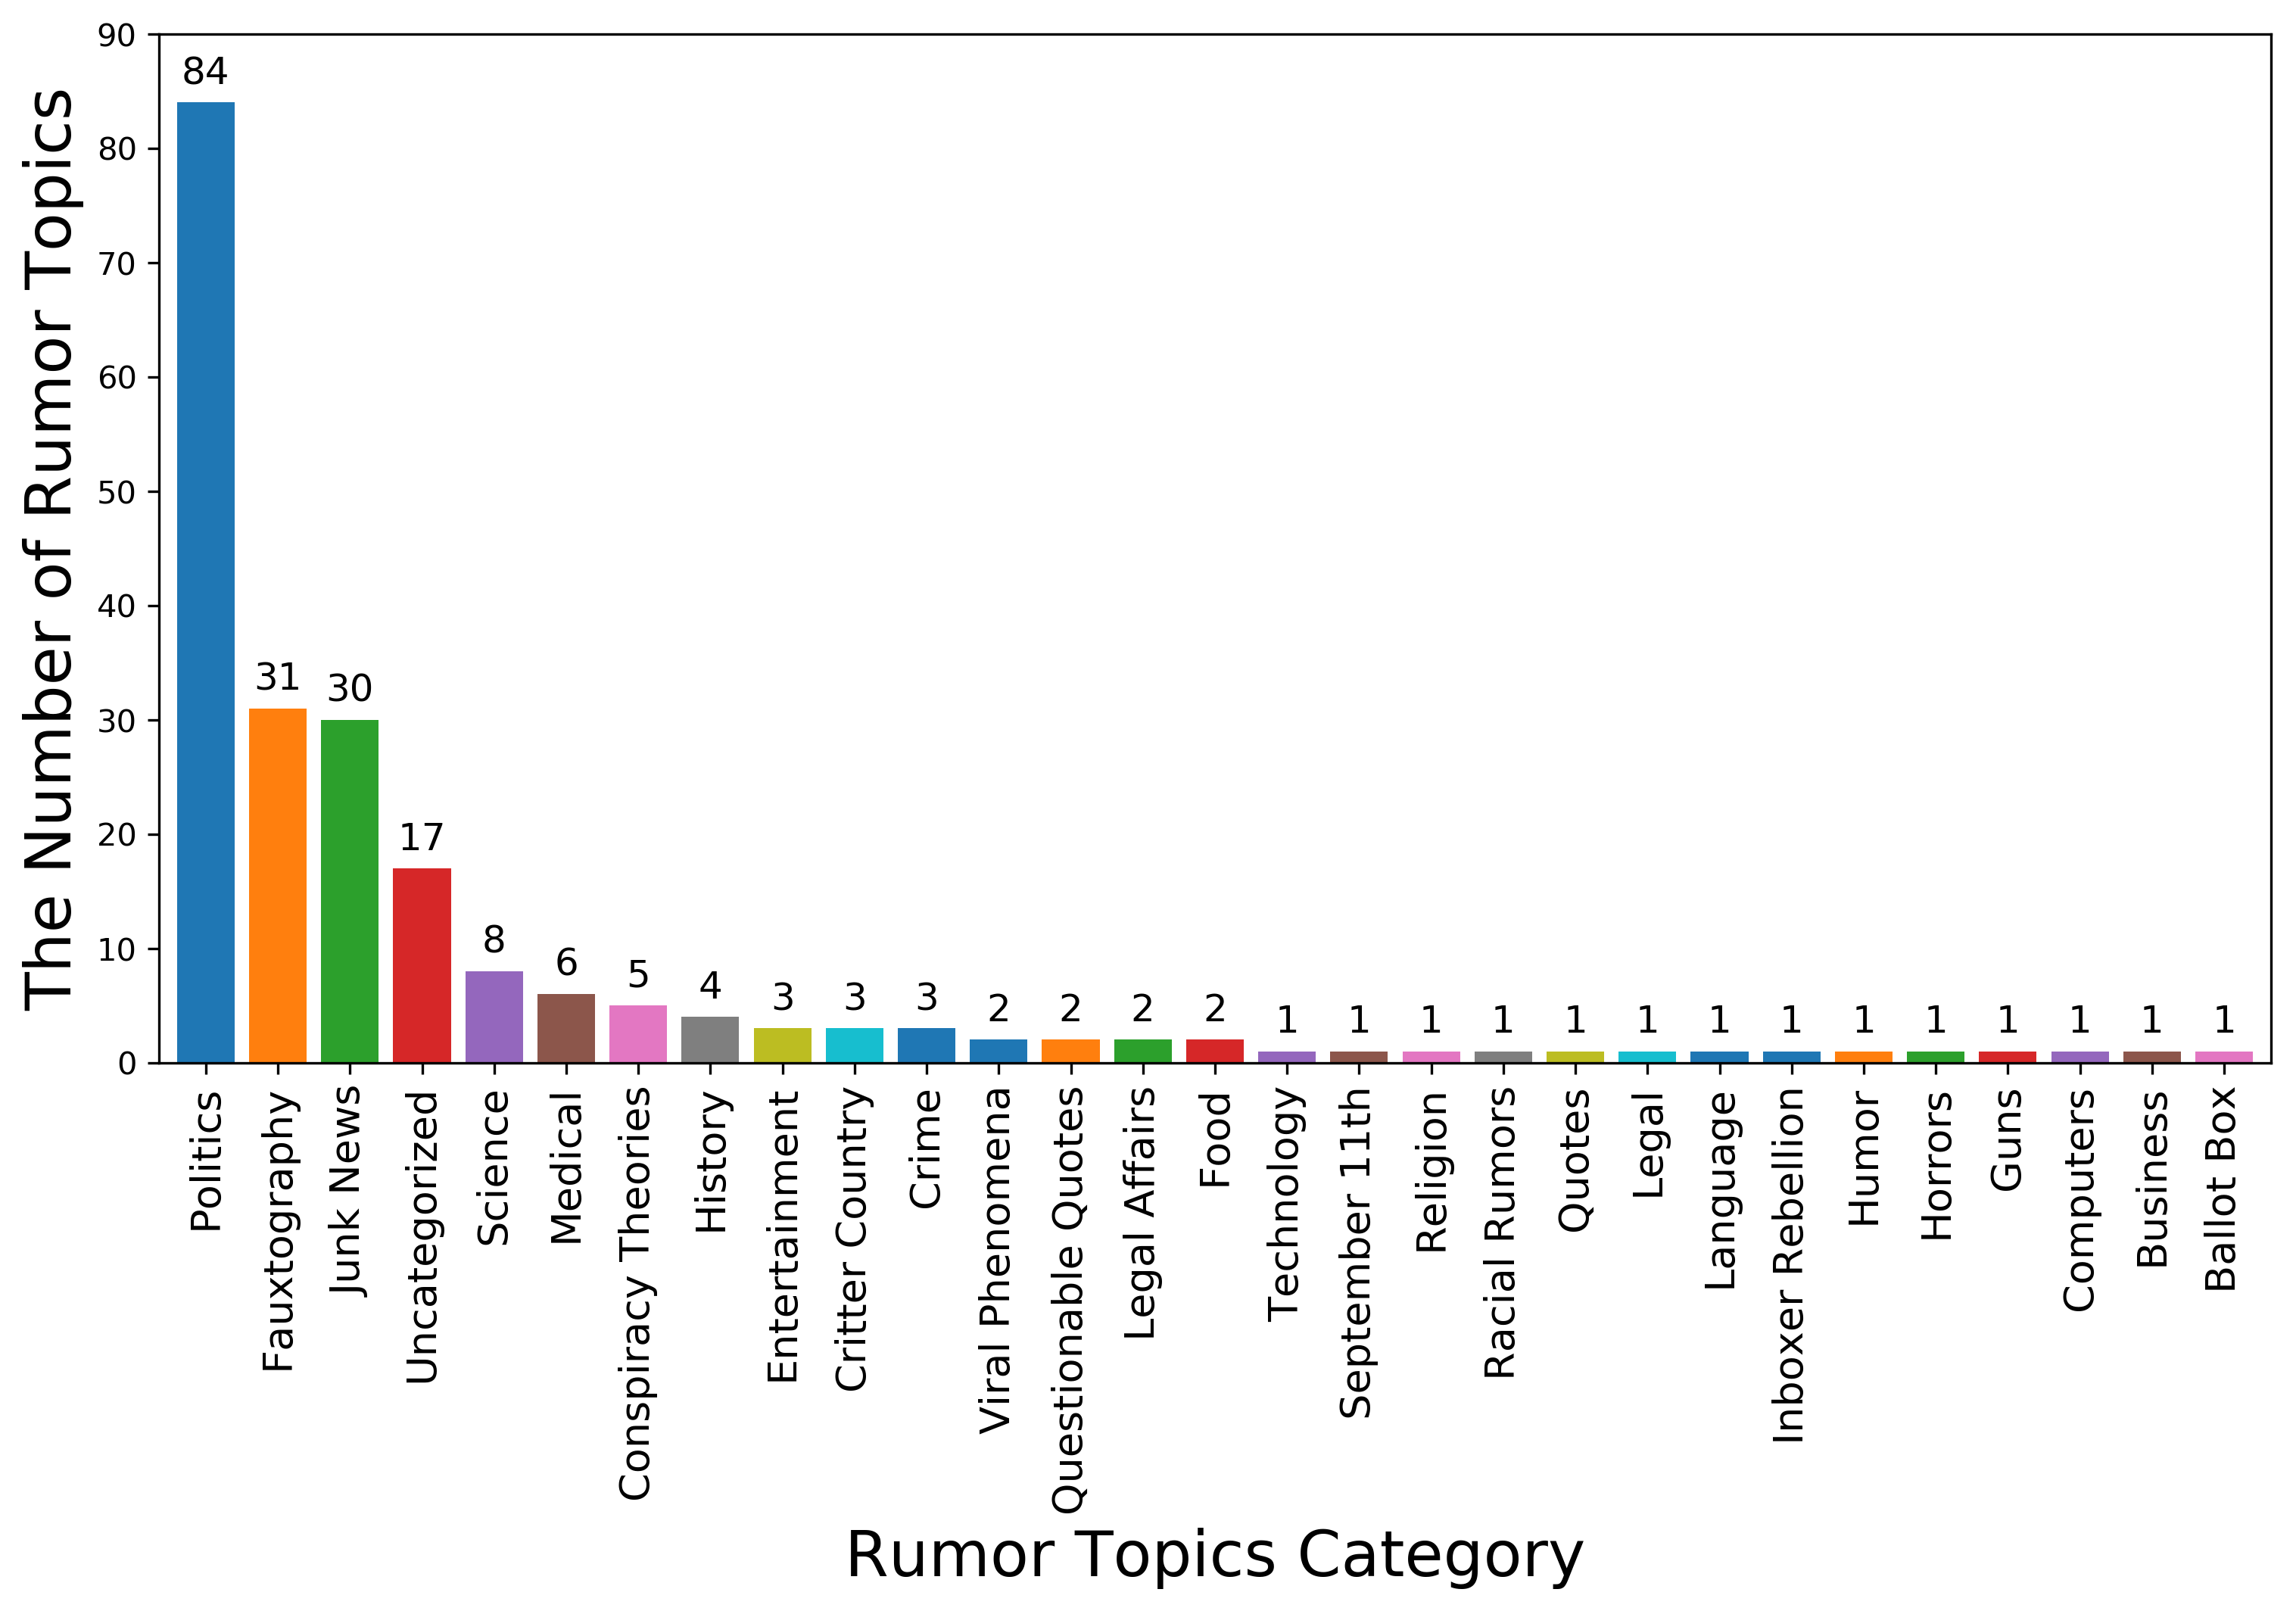
\includegraphics[width=3.3in]{figures/figure_1.png}}
		\caption{The number of rumor topics among categories on Snopes.com}
		\label{fig:bar_1}
	\end{figure}
	
	Furthermore, the study of veracity of online rumors have been conducted for a long time. According to Snopes, the veracity of total 216 rumor topics falls into three categories: there are 20\% of rumor topics marked as true by Snopes.com, and 58\% of rumor topics were considered as misinformation with its corresponding debunking source. The remaining rumor topics were labeled as Mostly True, Mostly False, Mixture, Unproven, or Miscaptioned, which means Snopes.com either found even portion of true and false information from the rumor topic or could not verify the credibility of the story. Note that we mark all rumor veracities other than absolute True or False as Mixture type for simplicity's sake. 
	
	We notice that the variance of the number of tweets per topic is relatively large, which brings up the problem of imbalance tweets amount among rumor topics. The average number of tweets for each topic is 1969. However, the maximum tweets amount of a topic is 50000 and the minimum is 102. What is striking in the minimum-size rumor topic is there are 98 out of 102 tweets are Snopes-related, namely the rumor-related tweets are far less than we anticipated. 
	
	To address the aforementioned imbalance problem, we further consider in two aspects - the validity of searching query and the higher re-share deletion rate of false rumor. In terms of the effectiveness of searching query, even though the searching queries were refined and reorganized by our tool, some searching queries still cannot efficiently find exact tweets set as manually specifying searching terms. On the other hand, false information have a higher probability of linking with debunking articles. Moreover, once it is linked with debunking information, there is a 4.4 times increase in deletion probability of false information, and the probability is even higher if the debunking information appear immediately after the false information \cite{friggeri2014rumor}. After examining all rumor topics with less than 500 acquired tweets, we found the number of true rumors is 12 out of 119, and the rest rumor topics' veracity is either false or mixture. The percentage of true rumors among total rumor topics with less than 500 acquired tweets is 10.08\%, while the proportion of true rumors in the whole dataset is 20.37\% (44 out of 216). The difference in the proportion of true rumors can explain the lack of tweets for some rumor topics from the side.
	
	
	\begin{table}[htbp]
		\caption{Statistics of the dataset}
		\begin{center}
			\begin{tabular}{|c|c|}
				\hline \\[-1em]
				Statistic           & Twitter Dataset \\
				\hline
				\\[-1em]
				\# of Users         & 221029          \\
				\hline
				\\[-1em]
				\# of Tweets        & 425333          \\
				\hline
				\\[-1em]
				\# of Topics        & 216             \\
				\hline
				\\[-1em]
				\# of True Rumors   & 44              \\
				\hline	
				\\[-1em]		
				\# of False Rumors  & 126             \\
				\hline	
				\\[-1em]		
				Max Tweets / Topics & 50000           \\
				\hline	
				\\[-1em]		
				Min Tweets / Topics & 102               \\
				\hline
			\end{tabular}
			\label{table: datasets}
		\end{center}
	\end{table}
	
	
	\section{The Role of Debunking Information}
	We set in motion to explore different aspects of a rumor's propagation on the online social network. To begin with, we delve into analyzing the different characteristics of the rumor's propagation. Furthermore, we examine the role of debunking information by considering the distribution of tweets amount of rumors and the statistical comparison of rumor cascades pre and post the debunking information. Above all, we wish to identify the mitigative effect of Snopes fact-checking message from comparing the tweets' sentimental change. 
	
	\subsection{The propagation of rumor on Twitter}
	
	%\begin{figure}[htbp]
	%	\centerline{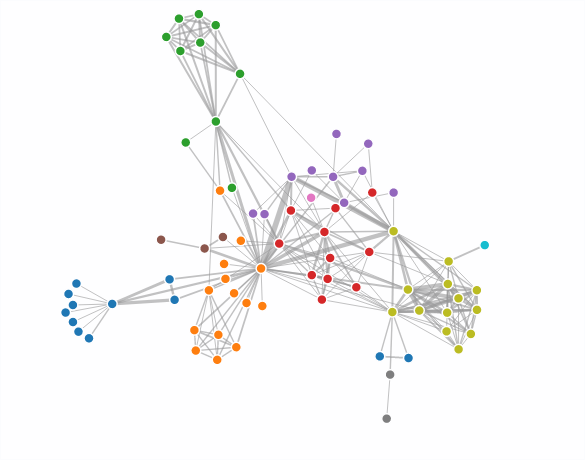
\includegraphics[width=3.2in]{figures/figure_3.png}}
	%	\caption{The distribution of the number of tweets of the rumor topic "Did Buzz Aldrin Say Not Punching Donald Trump Was His Greatest Achievement?"}
	%	\label{bar}
	%\end{figure}
	
	%\begin{figure}[htbp]
	%	\centerline{\includegraphics[width=3in,height=2in]{figures/figure_4.png}}
	%	\caption{TBD}
	%	\label{fig}
	%\end{figure}
	
	A rumor cascade typically starts with a statement about a topic on Twitter, and the main body of a rumor could include written text, photos, or links to articles online. Other users then propagate the rumor by resharing (retweeting) or replying it. In some cases, users on the social media platform may have a preference in some certain types of topics. As the Fig. \ref{fig:bar_1}
	
	Besides, the emerging time of top 216 rumor topics varies a lot, some topics were posted in 2016 or even later, which continues discussing heat during May to July 2017. Fig. \ref{fig:pie_1} shows the posting time distribution of our collected rumor topics. There are 89 rumor topics were posted before 2017, and nearly half of our collected tweets were discussed on the social network for over a year. Among the 89 topics, Politics is still the largest rumor category, followed by Fauxtography, Junk News, urban legend, categorized, and business. 
	
	\begin{figure}[htbp]
		\centerline{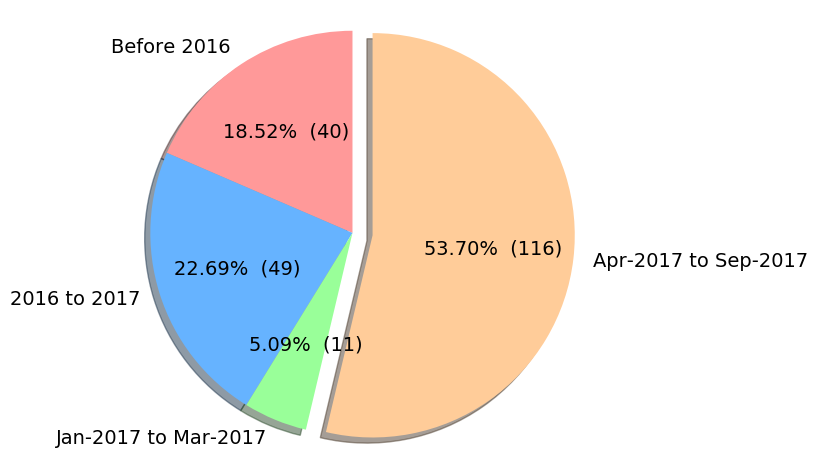
\includegraphics[width=3.2in]{figures/figure_2.png}}
		\caption{The Distribution of Rumor Topics Emerging Time}
		\label{fig:pie_1}
	\end{figure}
	
	For information that is sufficiently viral, it is highly possible that the influence of the rumor lasts for a long time on social media. We examine the 89 topics' veracity that originated before 2017, and the proportion of 89 rumor topics' veracity is approximately the same as the original 216 rumor topics. Therefore, the reason of perennial discussion of rumors is not because of rumor's veracity. 
	
	In this paper, we mainly focus on rumor cascades' variation in different time phases; particularly, we suspect there is a difference in the rumor cascade characteristics before and after the intervention of debunking information. Therefore, we name the rumor topics' appearing time within our searching time interval - April to September 2017, in order to compare pre and post characteristics change in rumor cascades. The resulting dataset contains 74 rumor topics and 233,223 related tweets. 
	
	\subsection{The Role of Debunking information}
	What effect does fact-checking information make in the rumor's dissemination process is still in doubt. We pay attention to the different distribution of the number of tweets in unit time before and after the debunking information, and we try to find a general trend that can fit and explain the tweets distribution. 
	
	Due to the average delay of at least 12 hours between the start of a rumor topic spread and that of its verifying information, false information tend to spread rapidly and widely during its starting phase \cite{kumar2016disinformation, zubiaga2016analysing}. Once fack-checking website like Snopes.com posts a debunking message, we want to know if the spread of the rumor topic will be mitigated. Taken the rumor topic "Clinton/Lynch Pilot Breaks His Silence on What Was Said?" as an example, it is evident that the number of tweets keeps growing in terms of individual days until the emerging of fact-checking information and the trend starts to decline after Snopes posted their fact-checking information (Fig \ref{fig:first_sub}). By observing the distribution after Snopes debunking information, we found there are high correlations between the distribution and chi-square distribution with 1 degree of freedom. 
	
	It's reasonable to suspect that the intervention of debunking information has a mitigating effect on the propagation of an online rumor since the debunking information posting time fall into the range of the peak of the distribution, and the distribution presents a downward trend after the posting of fact-checking information. The observed decrease in the distribution could be attributed to the posting of the debunking message. To further examine our hypothesis, we plot the normalized distribution Fig. \ref{fig:second_sub} (after smoothed the distribution graph in order to diminish the influence of the wave in distribution) along with the randomly generated chi-square distribution (Fig. \ref{fig:third_sub}), and rumor's distribution tends to have a similar trend with the chi-square distribution. The Kolmogorov-Smirnov Test (score=0.23809, p-value=0.15877) between two distributions also shows that our hypothesis cannot be rejected since p-value is greater than 0.05.
	
	Although the tweets distribution of the rumor from Fig. \ref{fig:second_sub} can fit the chi-square distribution, there are other rumor topics with various shape of distributions cannot fit a regular decreasing distribution. For the purpose of determining the decreasing trend of a rumor's tweets distribution after the intervention of debunking information, we proceed to examine the distribution of 74 rumor topics pre and post the intervention of fact-checking information. In specific, we transform and smooth the number of tweets before and after the Snopes message in terms of individual days to two separate arrays. If the distribution before the fact-checking information increases progressively increase while the distribution after the fact-checking information decreases progressively, we mark this rumor topic fitting the general trend that Snopes information can have a mitigative effect in the rumor's propagation. There are 70\% of the 74 rumors presenting the general upward and downward trend before and after the intervention of debunking information from the fact-checking website.
	
	\begin{figure}
		\centering
		\subfigure[Full Distribution of the Number of Tweets Per Day from 07/13/2017 to 08/28/2017]
		{
			\includegraphics[width=3in]{figures/figure_4A.png}
			\label{fig:first_sub}
		}
		\\
		\subfigure[The number of Tweets Distribution After Debunking Information]
		{
			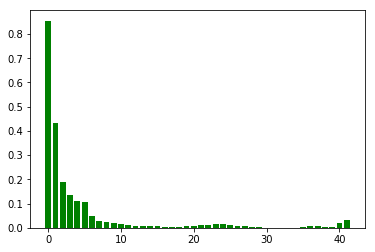
\includegraphics[width=1.6in]{figures/figure_4B.png}
			\label{fig:second_sub}
		}
		\subfigure[Randomly Generated Chi-Square Distribution with 1 degree of freedom]
		{
			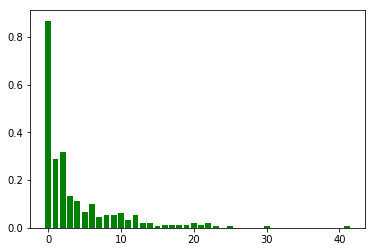
\includegraphics[width=1.6in]{figures/figure_4C.png}
			\label{fig:third_sub}
		}
		\caption{Distribution Comparison}
		\label{fig:distribution}
	\end{figure}
	
	\subsection{Statistical Analysis Before \& After Debunking Information}
	We have demonstrated the general impact of fact-checking information in the process of rumor diffusion, and a general statistical analysis can help us better understand how a piece of fact-checking information can change the propagation process. Besides, rumor cascades' characteristics can have a significant variation pre and post the fact-checking information. 
	
	We record the number of total tweets before and after Snopes's debunking information. By choosing the Snopes intervention time as the dividing point, 74 topics are partitioned into two groups. There are 29 rumor topics have more tweets before the posting of debunking information, and 45 topics have more tweets after the debunking information. The distribution of the rumor category for both sets are similar, and the most common categories are still Politics, Junk News, and Fauxtography. In contrast to category distribution, a significant difference has been found in the distribution of rumor veracity. Among all rumor topics with more tweets before Snopes information, there only exist "Mixture" and "False" rumors. In other words, people are more willing to discuss rumor topics that are verified as true by authorized social media after the fact-checking information, and misinformation and mixture rumors can draw more attention before the fact is checked.
	
	\begin{table}[htbp]
		\caption{Comparison of Before and After Fact-checking}
		\begin{center}
			\begin{tabular}{|c|c|c|}
				\hline \\[-1em]
				& Before Fact-checking & After Fact-checking \\ \hline \\[-1em]
				Total \# of Retweets       & 107963   & 65124 \\ \hline \\[-1em]
				Average \# of Retweets     & 1384.14    & 834.92    \\ \hline \\[-1em]
				Total \# of Users & 72299   & 51223      \\ \hline \\[-1em]
				Total \# of Cascades & 23964   & 27456      \\ \hline \\[-1em]
				Average \# of Cascades &  307.23  & 352.00      \\ \hline \\[-1em]
				Max Size of Cascades &  2863  & 2369      \\ \hline \\[-1em]
				Min Size of Cascades &  3  & 2      \\ \hline \\[-1em]
				Average Size of Cascades &  4.79  & 3.63      \\ \hline
			\end{tabular}
			\label{tab1e:debunking}
		\end{center}
	\end{table}
	
	Table \ref{tab1e:debunking} compares the summary statistics of the rumors' propagation characteristics before and after the debunking information. What can be clearly seen in the table is the significant difference between the statistics before and after the rumor is fact-checked. A rumor draws numerous users' notices (the number of retweets/replies and the number of involved users) until fact-checking media like Snopes.com posts the debunking information, which reflects the role of fact-checking information in controlling the spread of online rumors no matter whether rumors are verified as True or False from different perspectives. 
	
	In addition, by following  Vosoughi et al's definition: there can exist one or more \textbf{\emph{cascades}} in a rumor's diffusion process, which we define as instances of a rumor-spreading pattern that exhibit an unbroken re-tweet chain with a common, singular origin \cite{vosoughi2018spread}. In the dataset, differences of rumor cascades can also be found in a number of important aspects before and after the fact-checking message. Although the number of total cascades after the fact-checking message is greater than the number before the message, the maximum and minimum size of cascades before the fact-checking are 23964 and 3 among 74 rumor topics, while the number of maximum and minimum cascades' size after the Snopes debunking information are 2369 and 2, respectively. Considering there exist overlapped cascades across the debunking information; in other words, same cascades may keep growing after the posting of debunking information. By excluding the overlapped part, the total number of cascades formed before the intervention of the fact-checking website is 13532, and the number of newly emerged cascades after the debunking information is 12312. Therefore, the alleviating effect of fact-checking information in the spread of rumors is backed up by the results. 
	
	\begin{figure}[htbp]
		\centerline{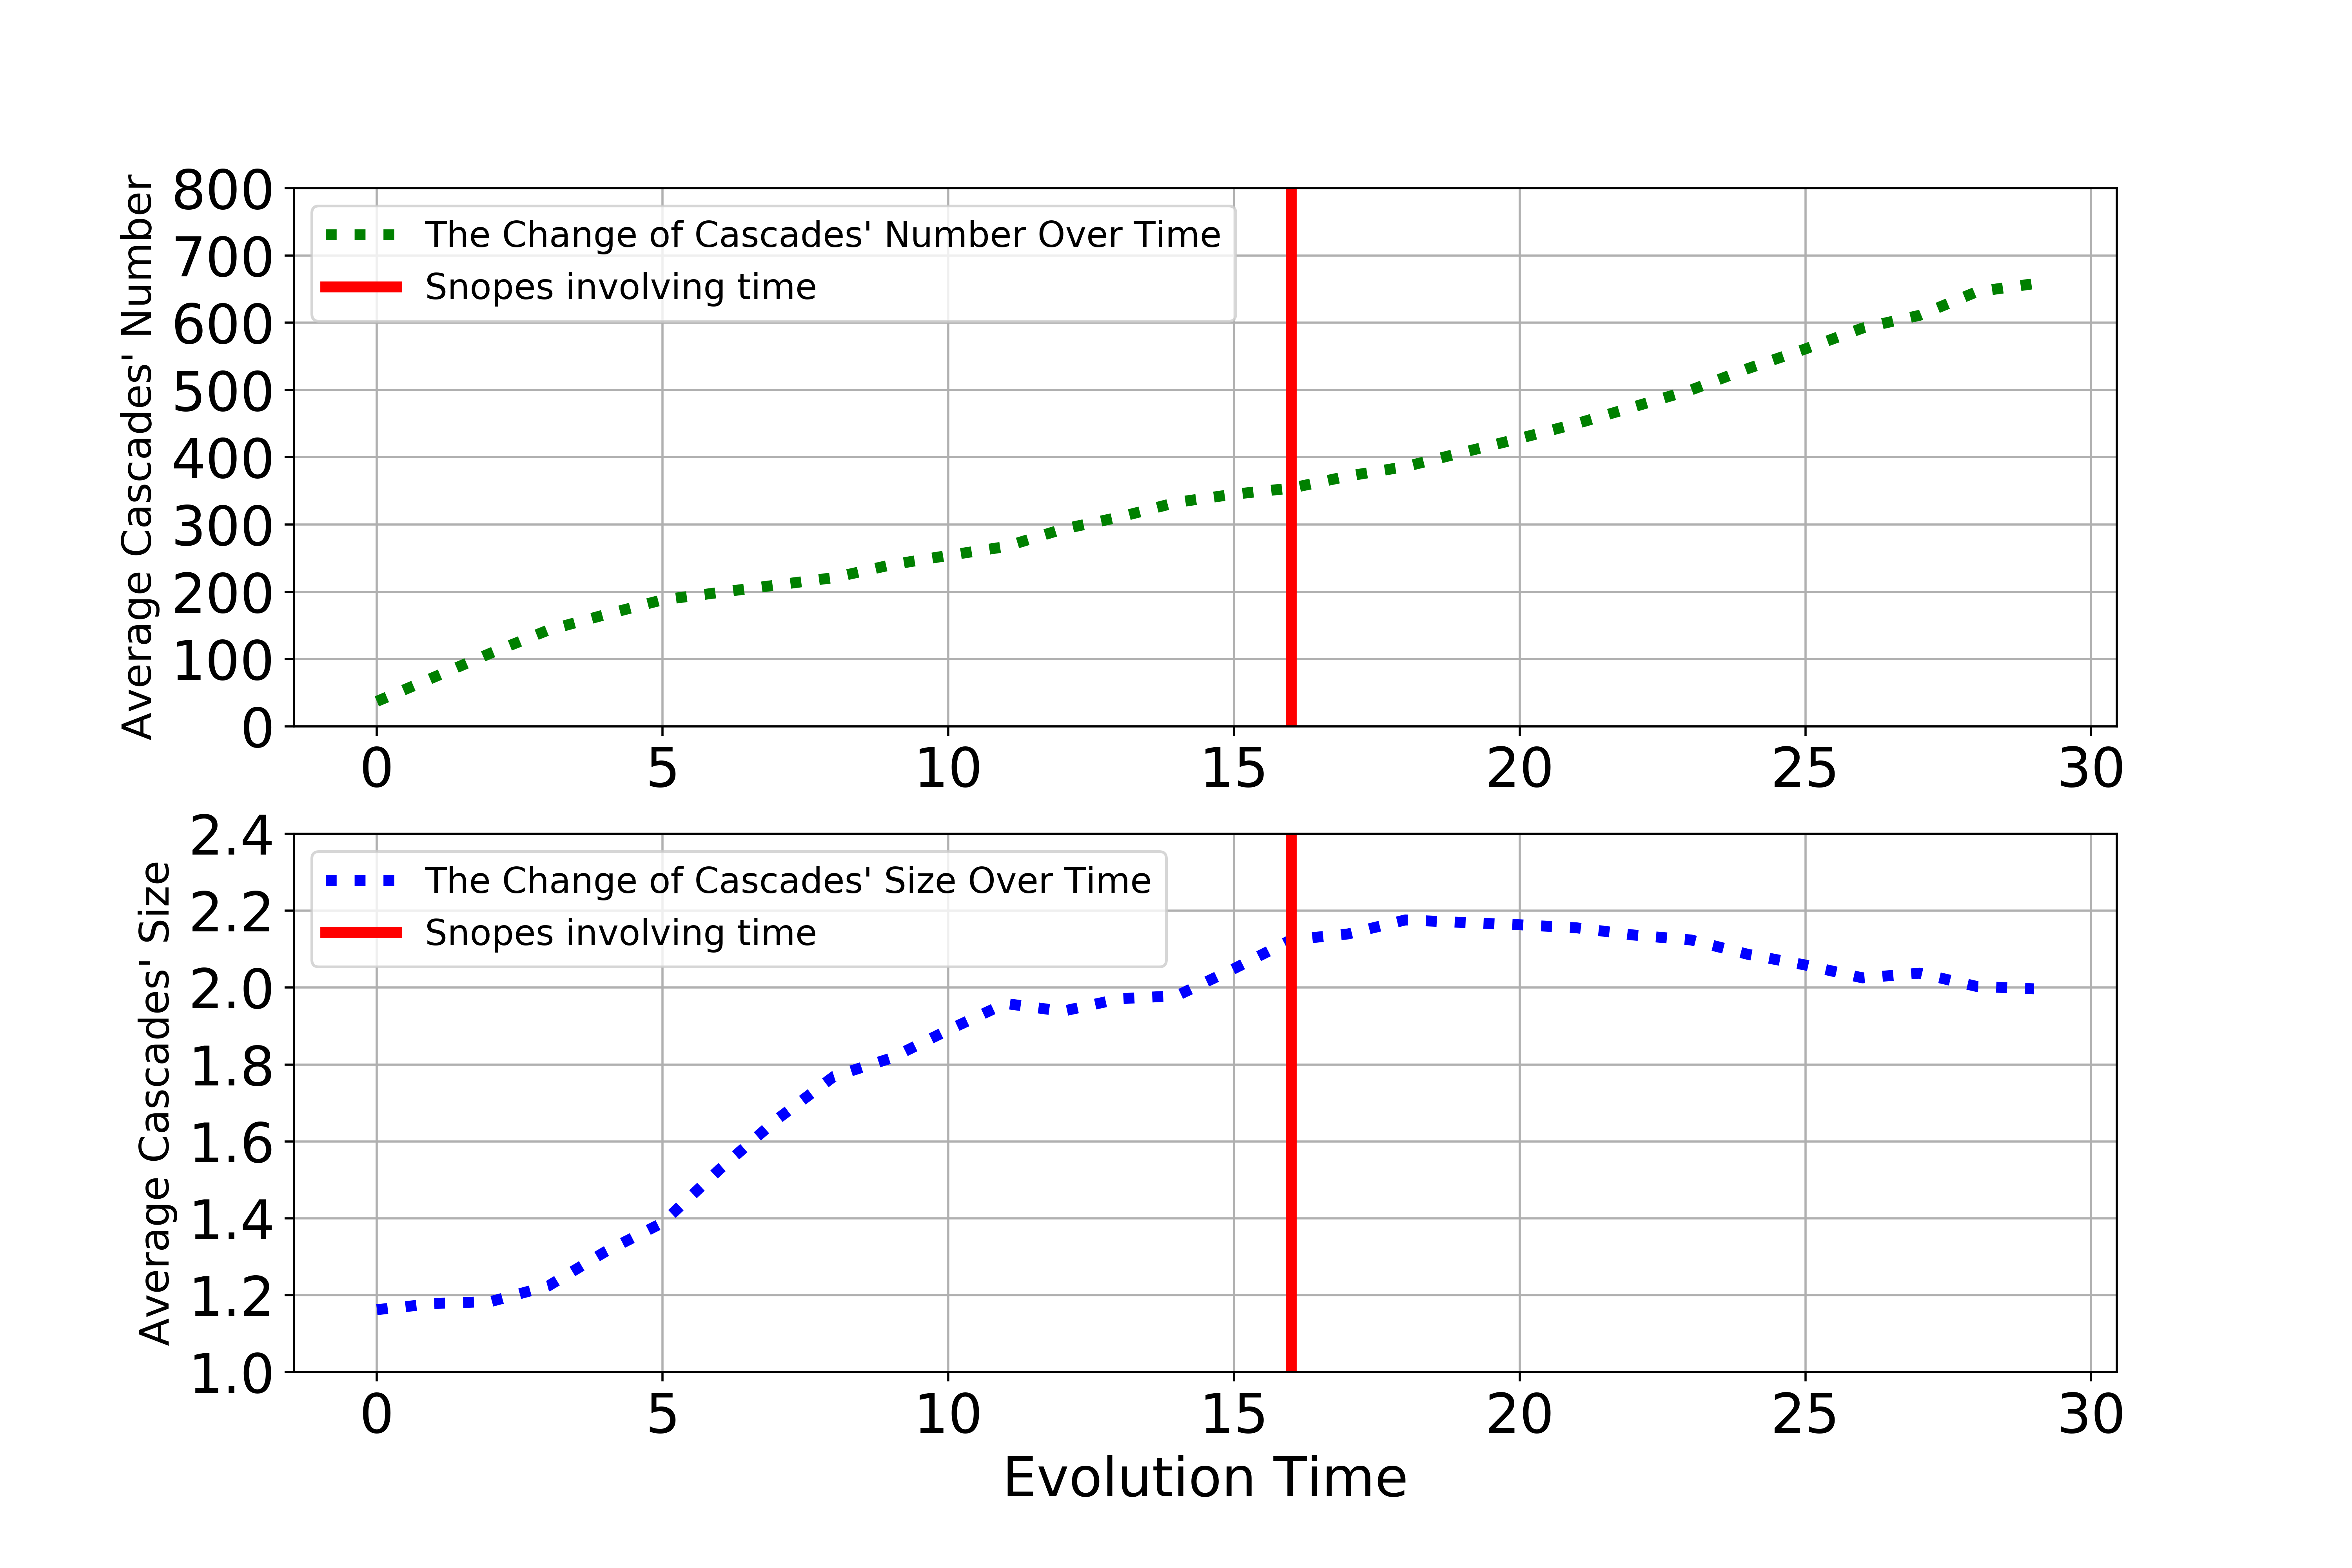
\includegraphics[width=3.7in]{figures/figure_5.png}}
		\caption{The Cascades Evolution of Rumor Topic 'Clinton/Lynch Pilot Breaks His Silence on What Was Said?' Over Time}
		\label{fig:evolution}
	\end{figure}
	
	Fig. \ref{fig:evolution} presents the cascades' evolution in the propagation of the aforementioned rumor topic 'Clinton/Lynch Pilot Breaks His Silence on What Was Said?'. The graph shows that there has been a relatively stable growth in the total number of cascades over time, and it reaches 658 individual rumor cascades at the end of the propagation. As can be seen from the graph, although the debunking information does not disturb the smoothly increasing trend of the total number of cascades, the average size of cascades are impacted by the debunking message. The posting of the fact-checking information is the turning point of the growth of the cascades' average size. The cascades' size begins to drop at 2.169 after the intervention of debunking information. As stated in \cite{friggeri2014rumor} and \cite{zubiaga2016analysing}, after presenting the corrective information of fake news, there are still a small fraction of users denying the debunking articles, and there is a higher probability that users would delete their previous retweets or replies of the false information and retweet debunking information of the fake news. Therefore, yet the amount of cascades is still growing, the cascade's size drops after the debunking information. Even though a small fraction of users are still tweeting either supportive or denying tweets, those tweets cannot form a large cascade because the influence of rumor decrease and it cannot affect other users after the revealing of debunking information. Therefore, after fact-checking website posts the verifying information, a rumor is still able to disseminate deeper in the social network; however, it loses the ability to affect broader users at the final phase of the propagation. 
	
	\begin{figure*}[htp]
		\centering
		\subfigure[Before Debunking Message]
		{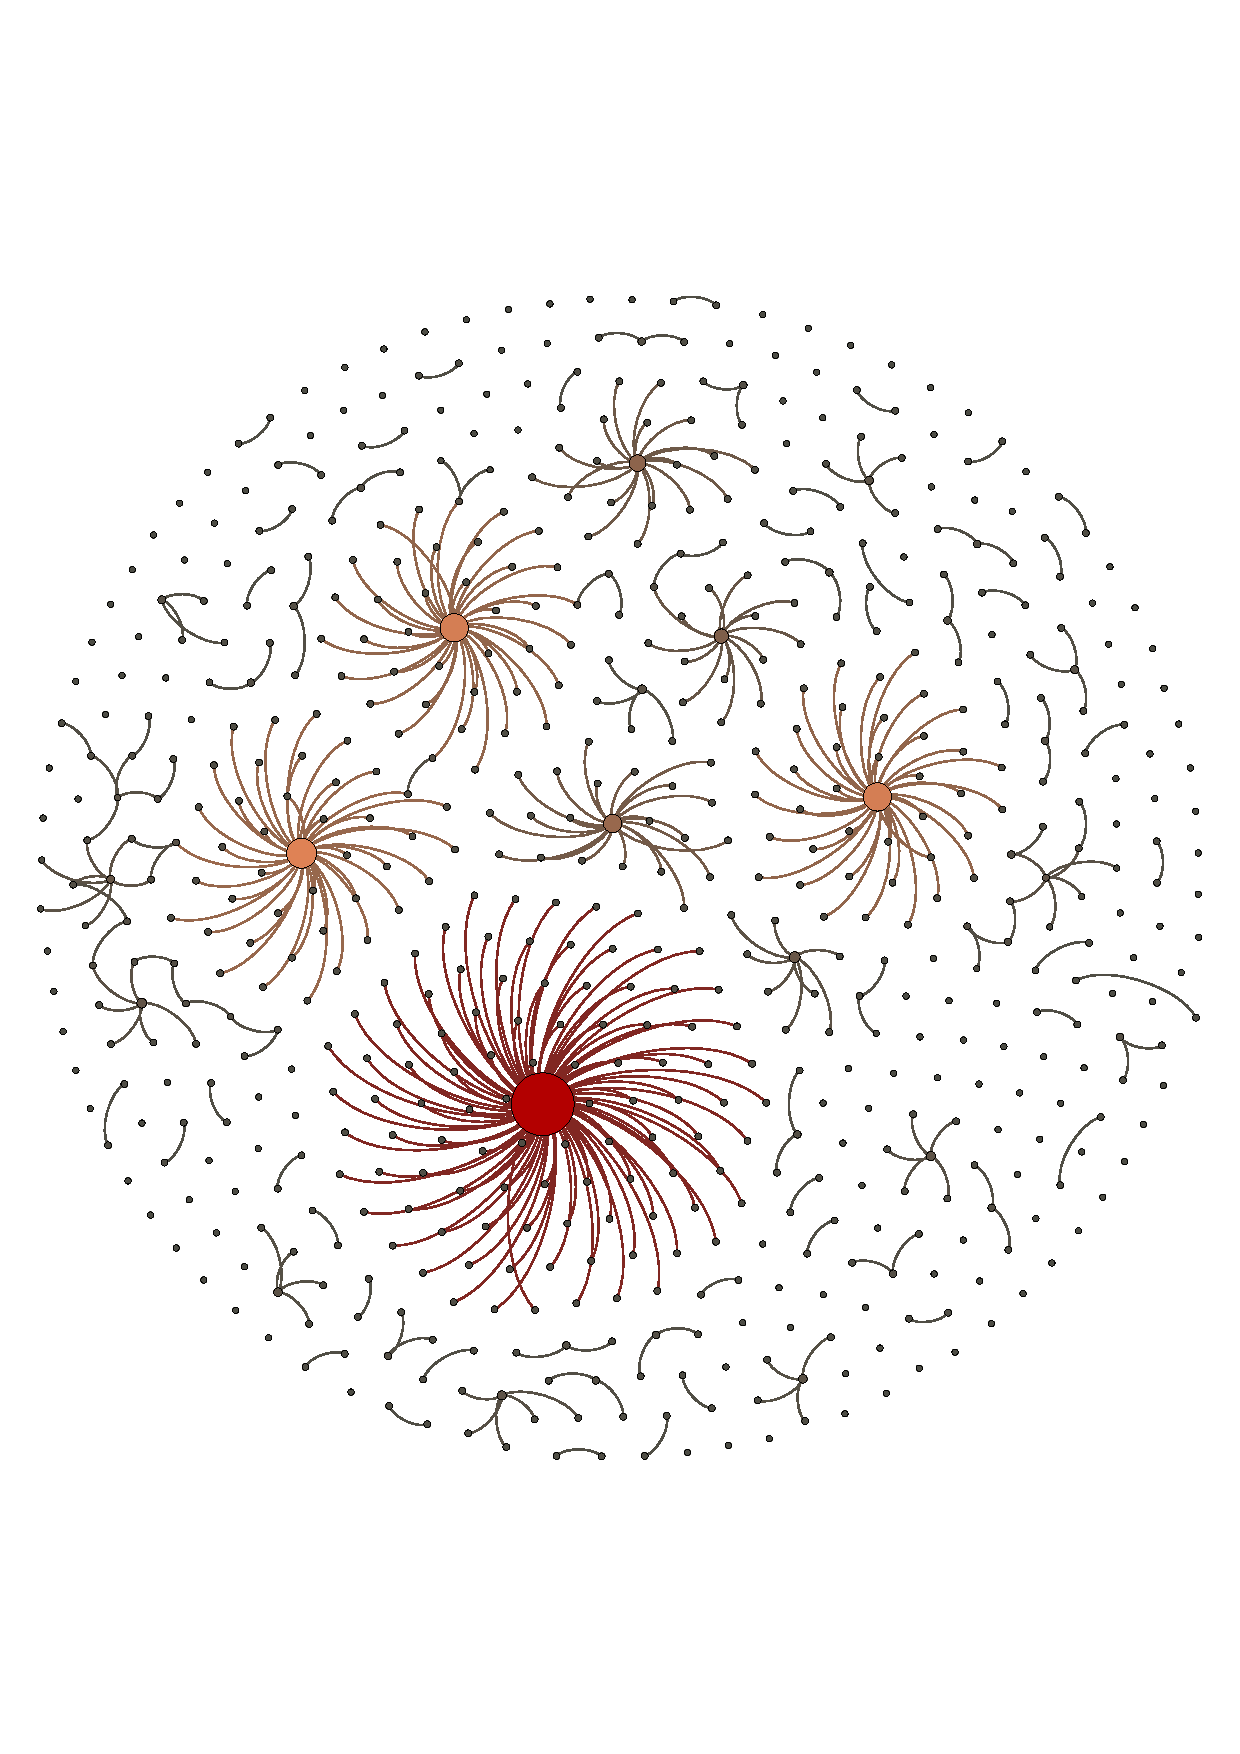
\includegraphics[scale=0.33]{figures/before.pdf}
			\label{fig:prop_first_sub}}\quad
		\subfigure[After Debunking Information]
		{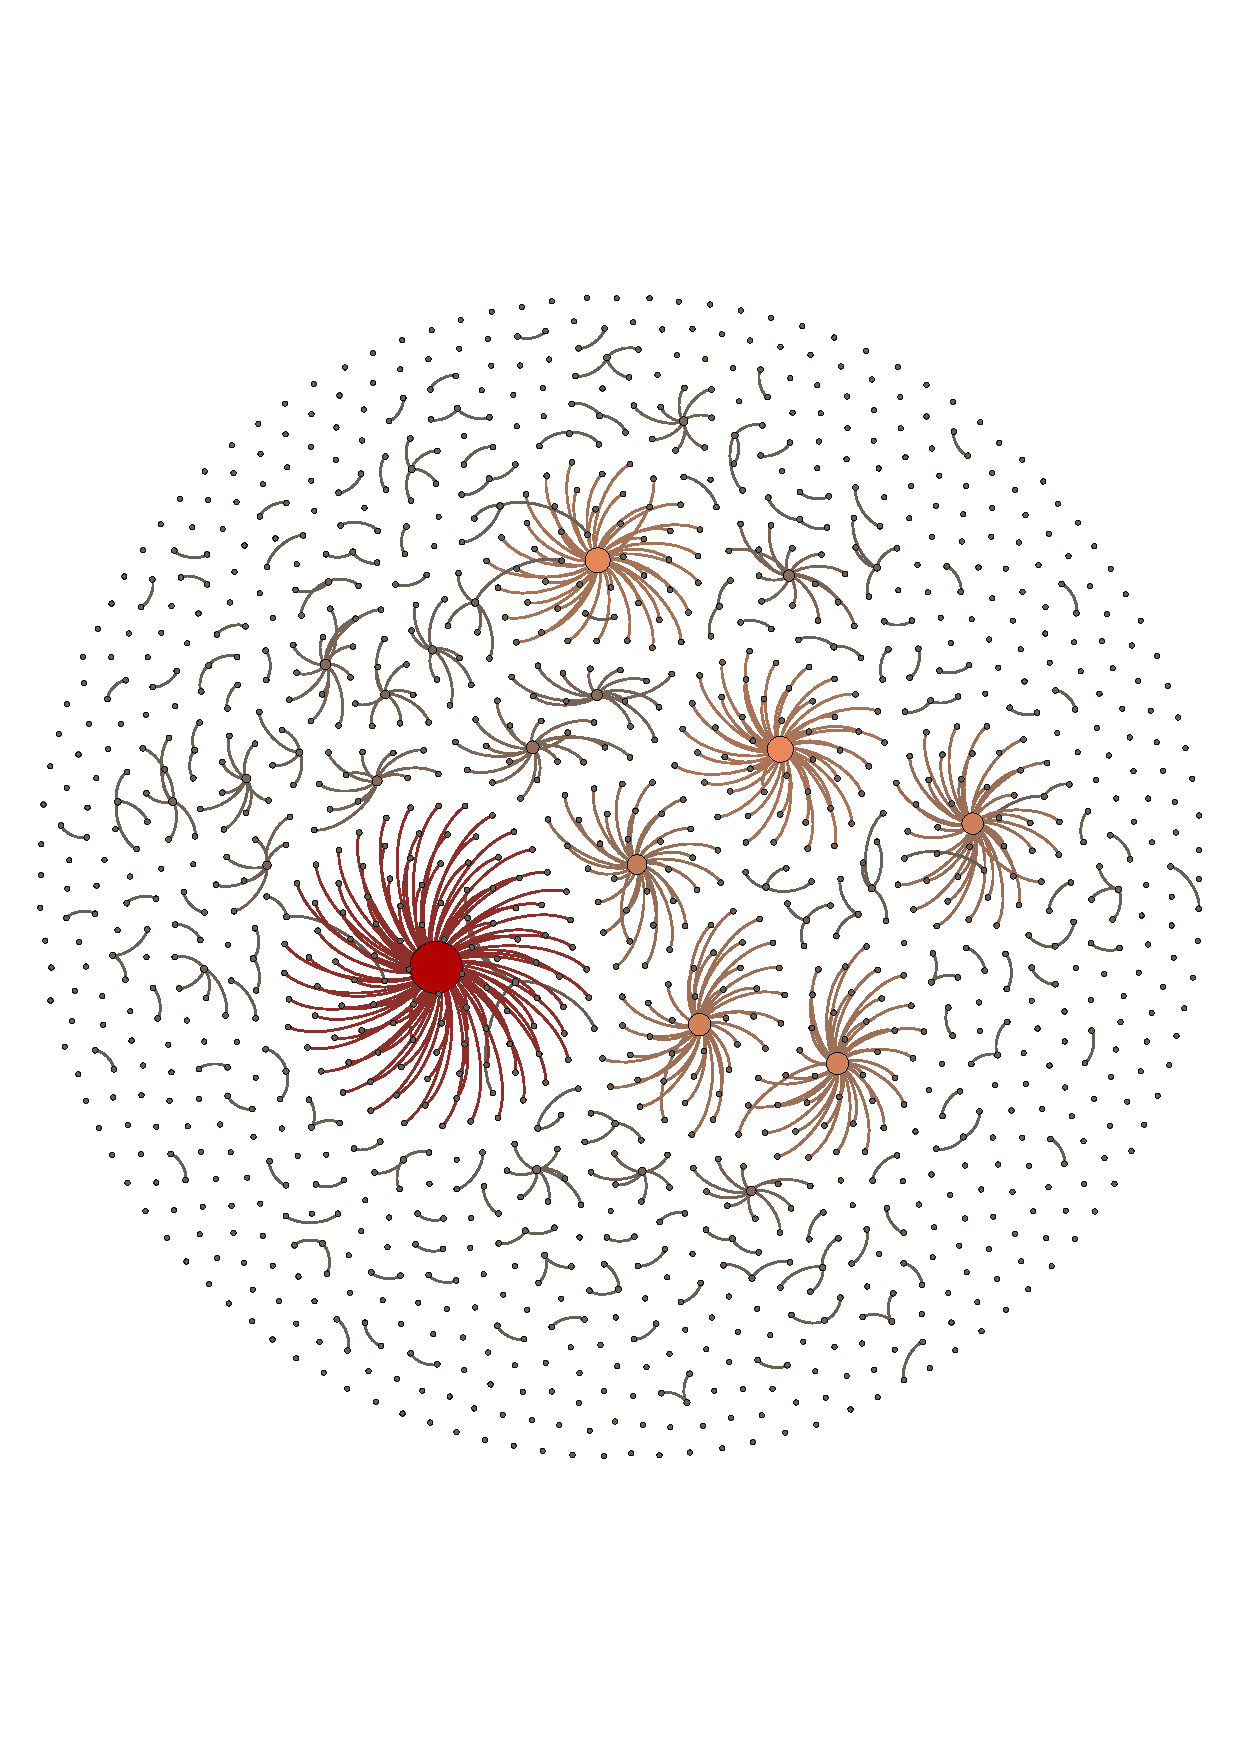
\includegraphics[scale=0.33]{figures/all.pdf}
			\label{fig:prop_second_sub}}
		\caption{An illustrative example of Rumor Propagation on Twitter.}
		\label{fig:propagation}
		\vspace{-3mm}
	\end{figure*}
	
	Figure \ref{fig:propagation} illustratively exposes the cascade evolution of the rumor topic - 'Clinton/Lynch Pilot Breaks His Silence on What Was Said?'. Fig. \ref{fig:prop_first_sub} and Fig. \ref{fig:prop_second_sub} exhibit the cascades propagation before the fact-checking information and the comprehensive cascades propagation of the rumor topic, respectively. In Fig. \ref{fig:prop_first_sub}, the number of nodes and edges are 638 and 431, and the number of nodes and edges are 1336 and 693 in Fig. \ref{fig:prop_second_sub}. In the undirected graphs, each node represents an individual Twitter user, and an edge between every two nodes represents the user either retweeted, replied, or quoted the other user's tweets. A node's color and size is ranked by its degree. The redder and bigger a node, the degree of the node is larger, and there are more surrounding nodes. 
	
	As we mentioned previously in Fig. \ref{fig:evolution}, a rumor generally can spread rapidly at its early phase. Several comparatively large cascades are generated before the posting of debunking information. However, after the intervention of debunking information, a rumor loses its ability to affect broader users since the average size of cascades drops while the total number of cascades keeps increasing. The number of involved users doubles between two propagation phases, but the increase of edges number is limited, which suggests that the graph turns to be less connected because of the lack of users' re-shares. Similarly, it can be seen from the trend in Fig. \ref{fig:prop_second_sub} that nearly no large cascades formed comparing with Fig. \ref{fig:prop_first_sub}. Conversely, a number of single cascades are formed after the posting of debunking information. Statistics of the graph also points out that the average degree in Fig. \ref{fig:prop_first_sub} is 1.531 while the average degree is 1.137 in Fig. \ref{fig:prop_second_sub}. After checking those single cascades' tweet, a large fraction of the content is about debunking information. Therefore, the posting of fact-checking information can limit the spread of rumor, and users also show fewer interests in spreading rumor after it has been verified. Next, it is imperative to consider the user's attitude switch pre and post the fact-checking information. 
	
	
	\subsection{Sentiment Analysis Before \& After Debunking Information}
	
	\begin{figure}[htp]
		\centering
		\subfigure[User's Attitudes Evolution Over Time of Rumor topic]
		{
			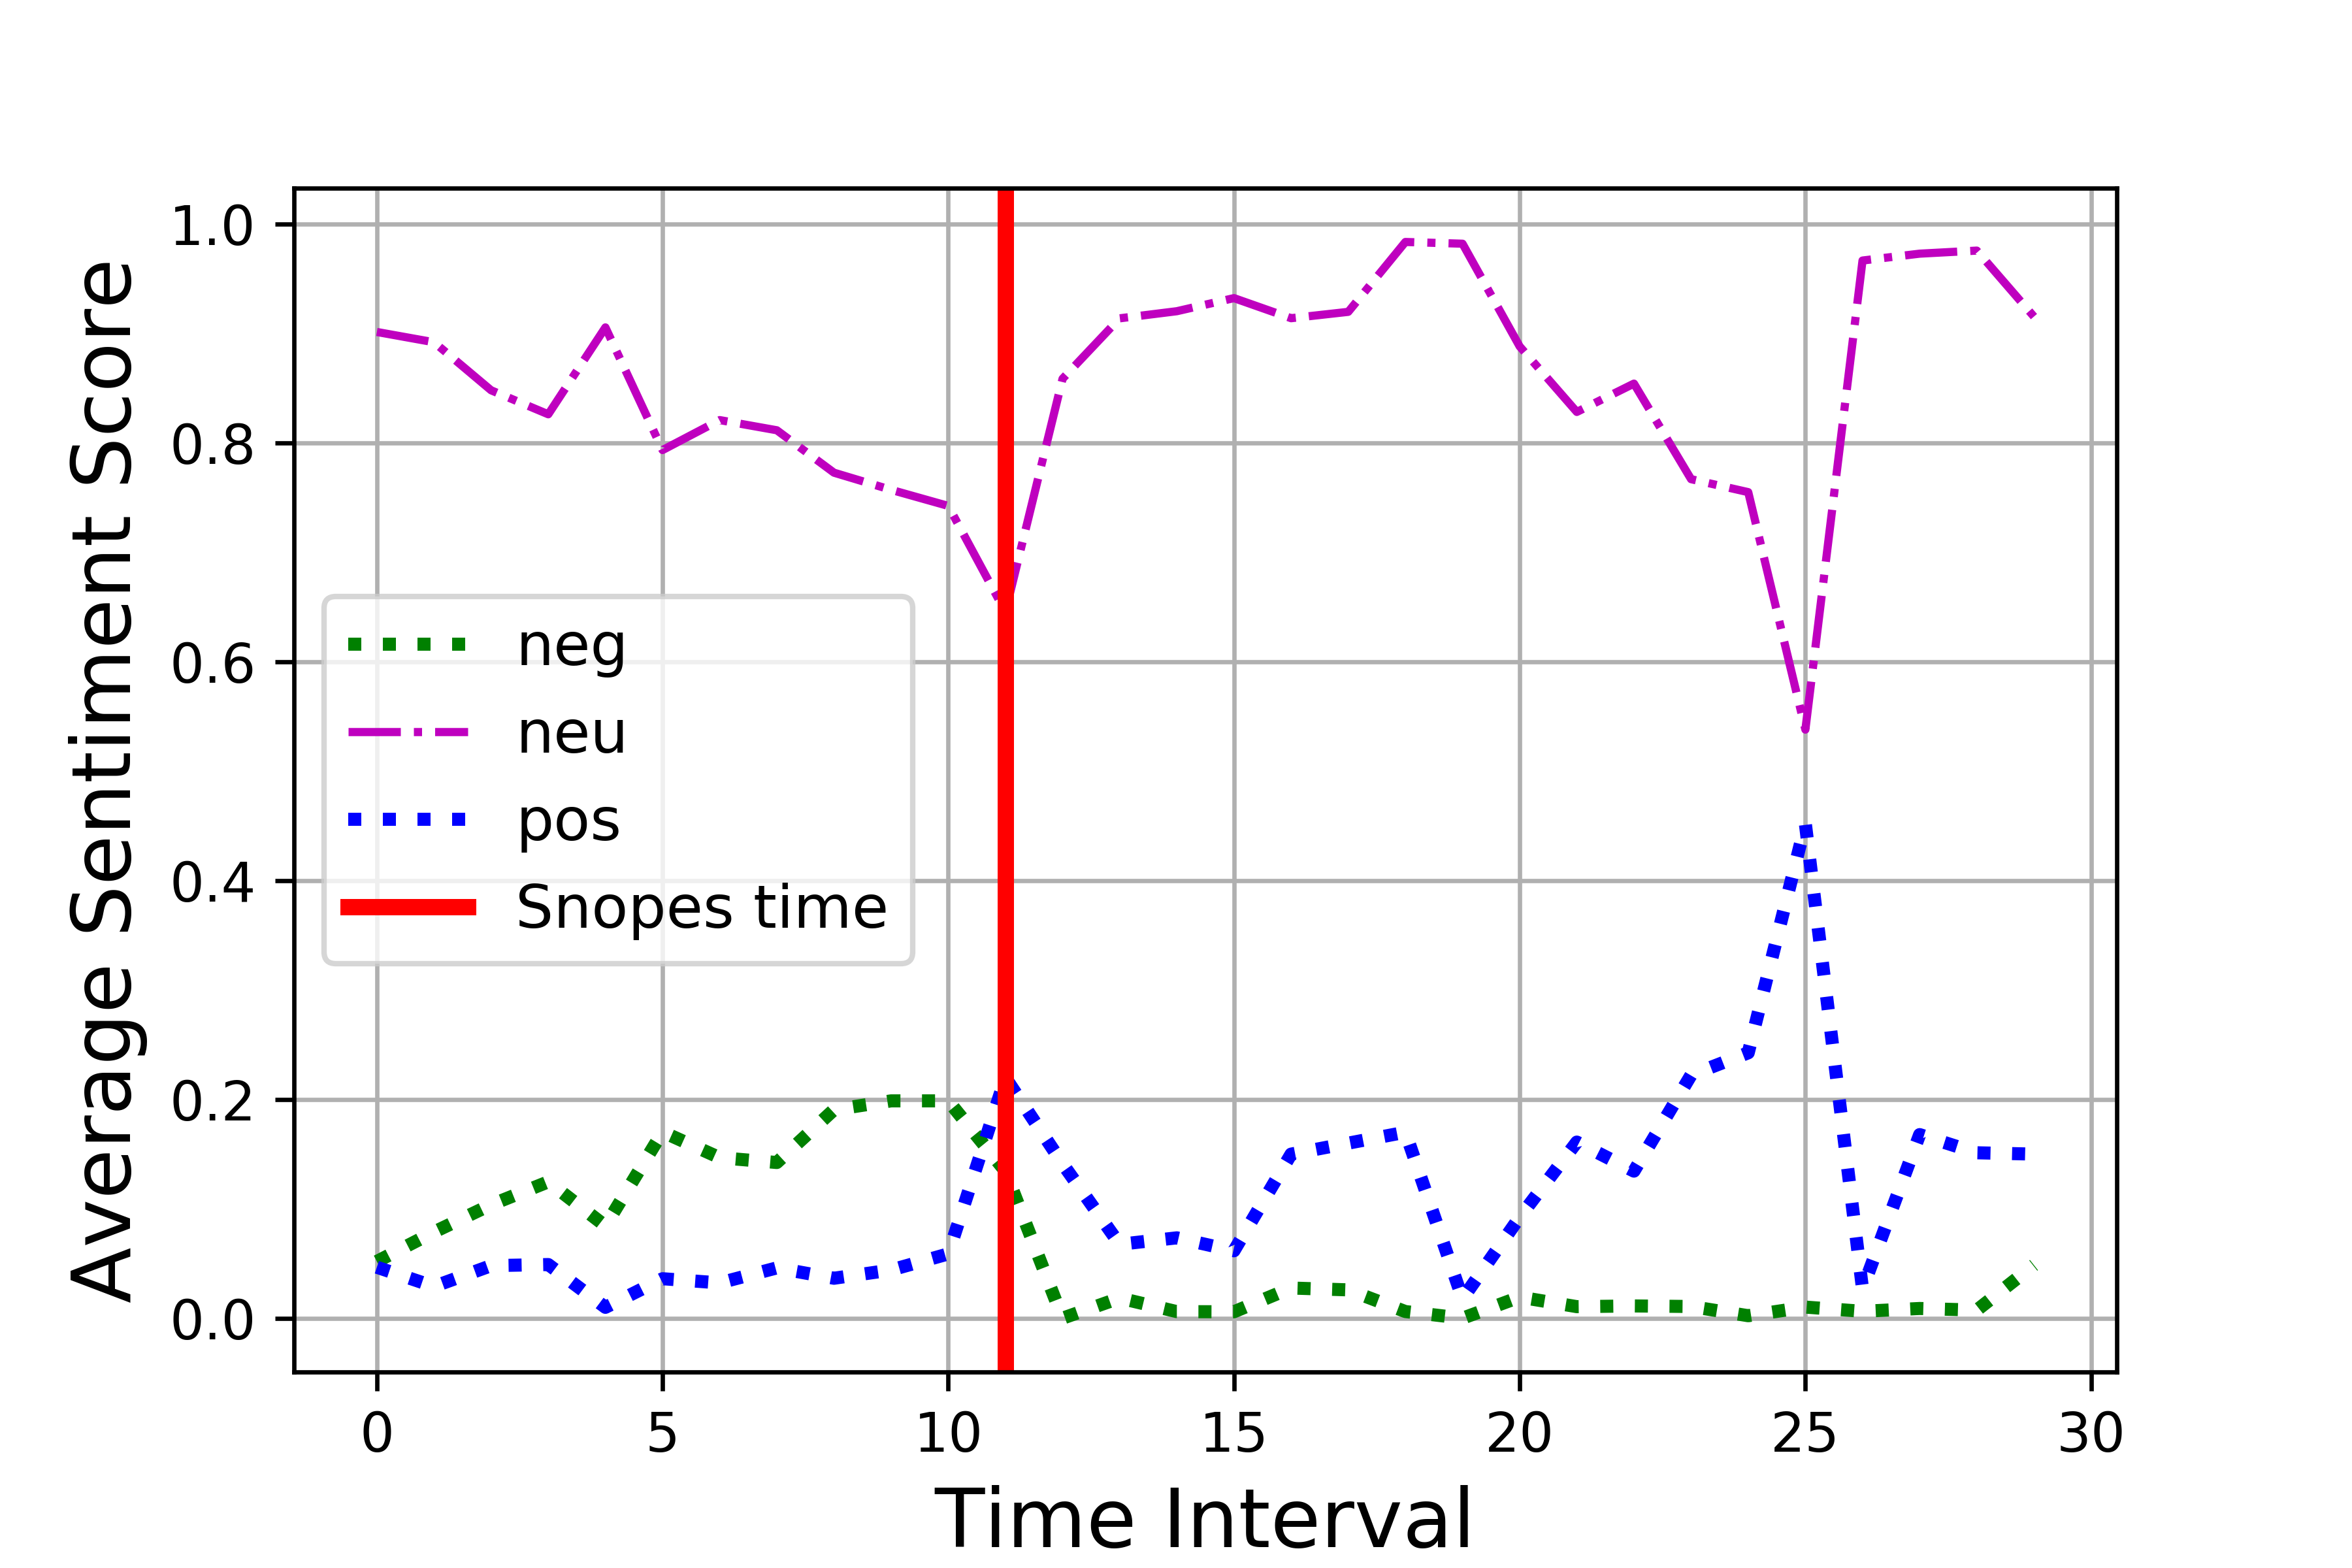
\includegraphics[width=3in]{figures/figure_6A.png}
			\label{fig:att_first_sub}
		}
		\subfigure[Overall Sentiment Score Change Over Time]
		{
			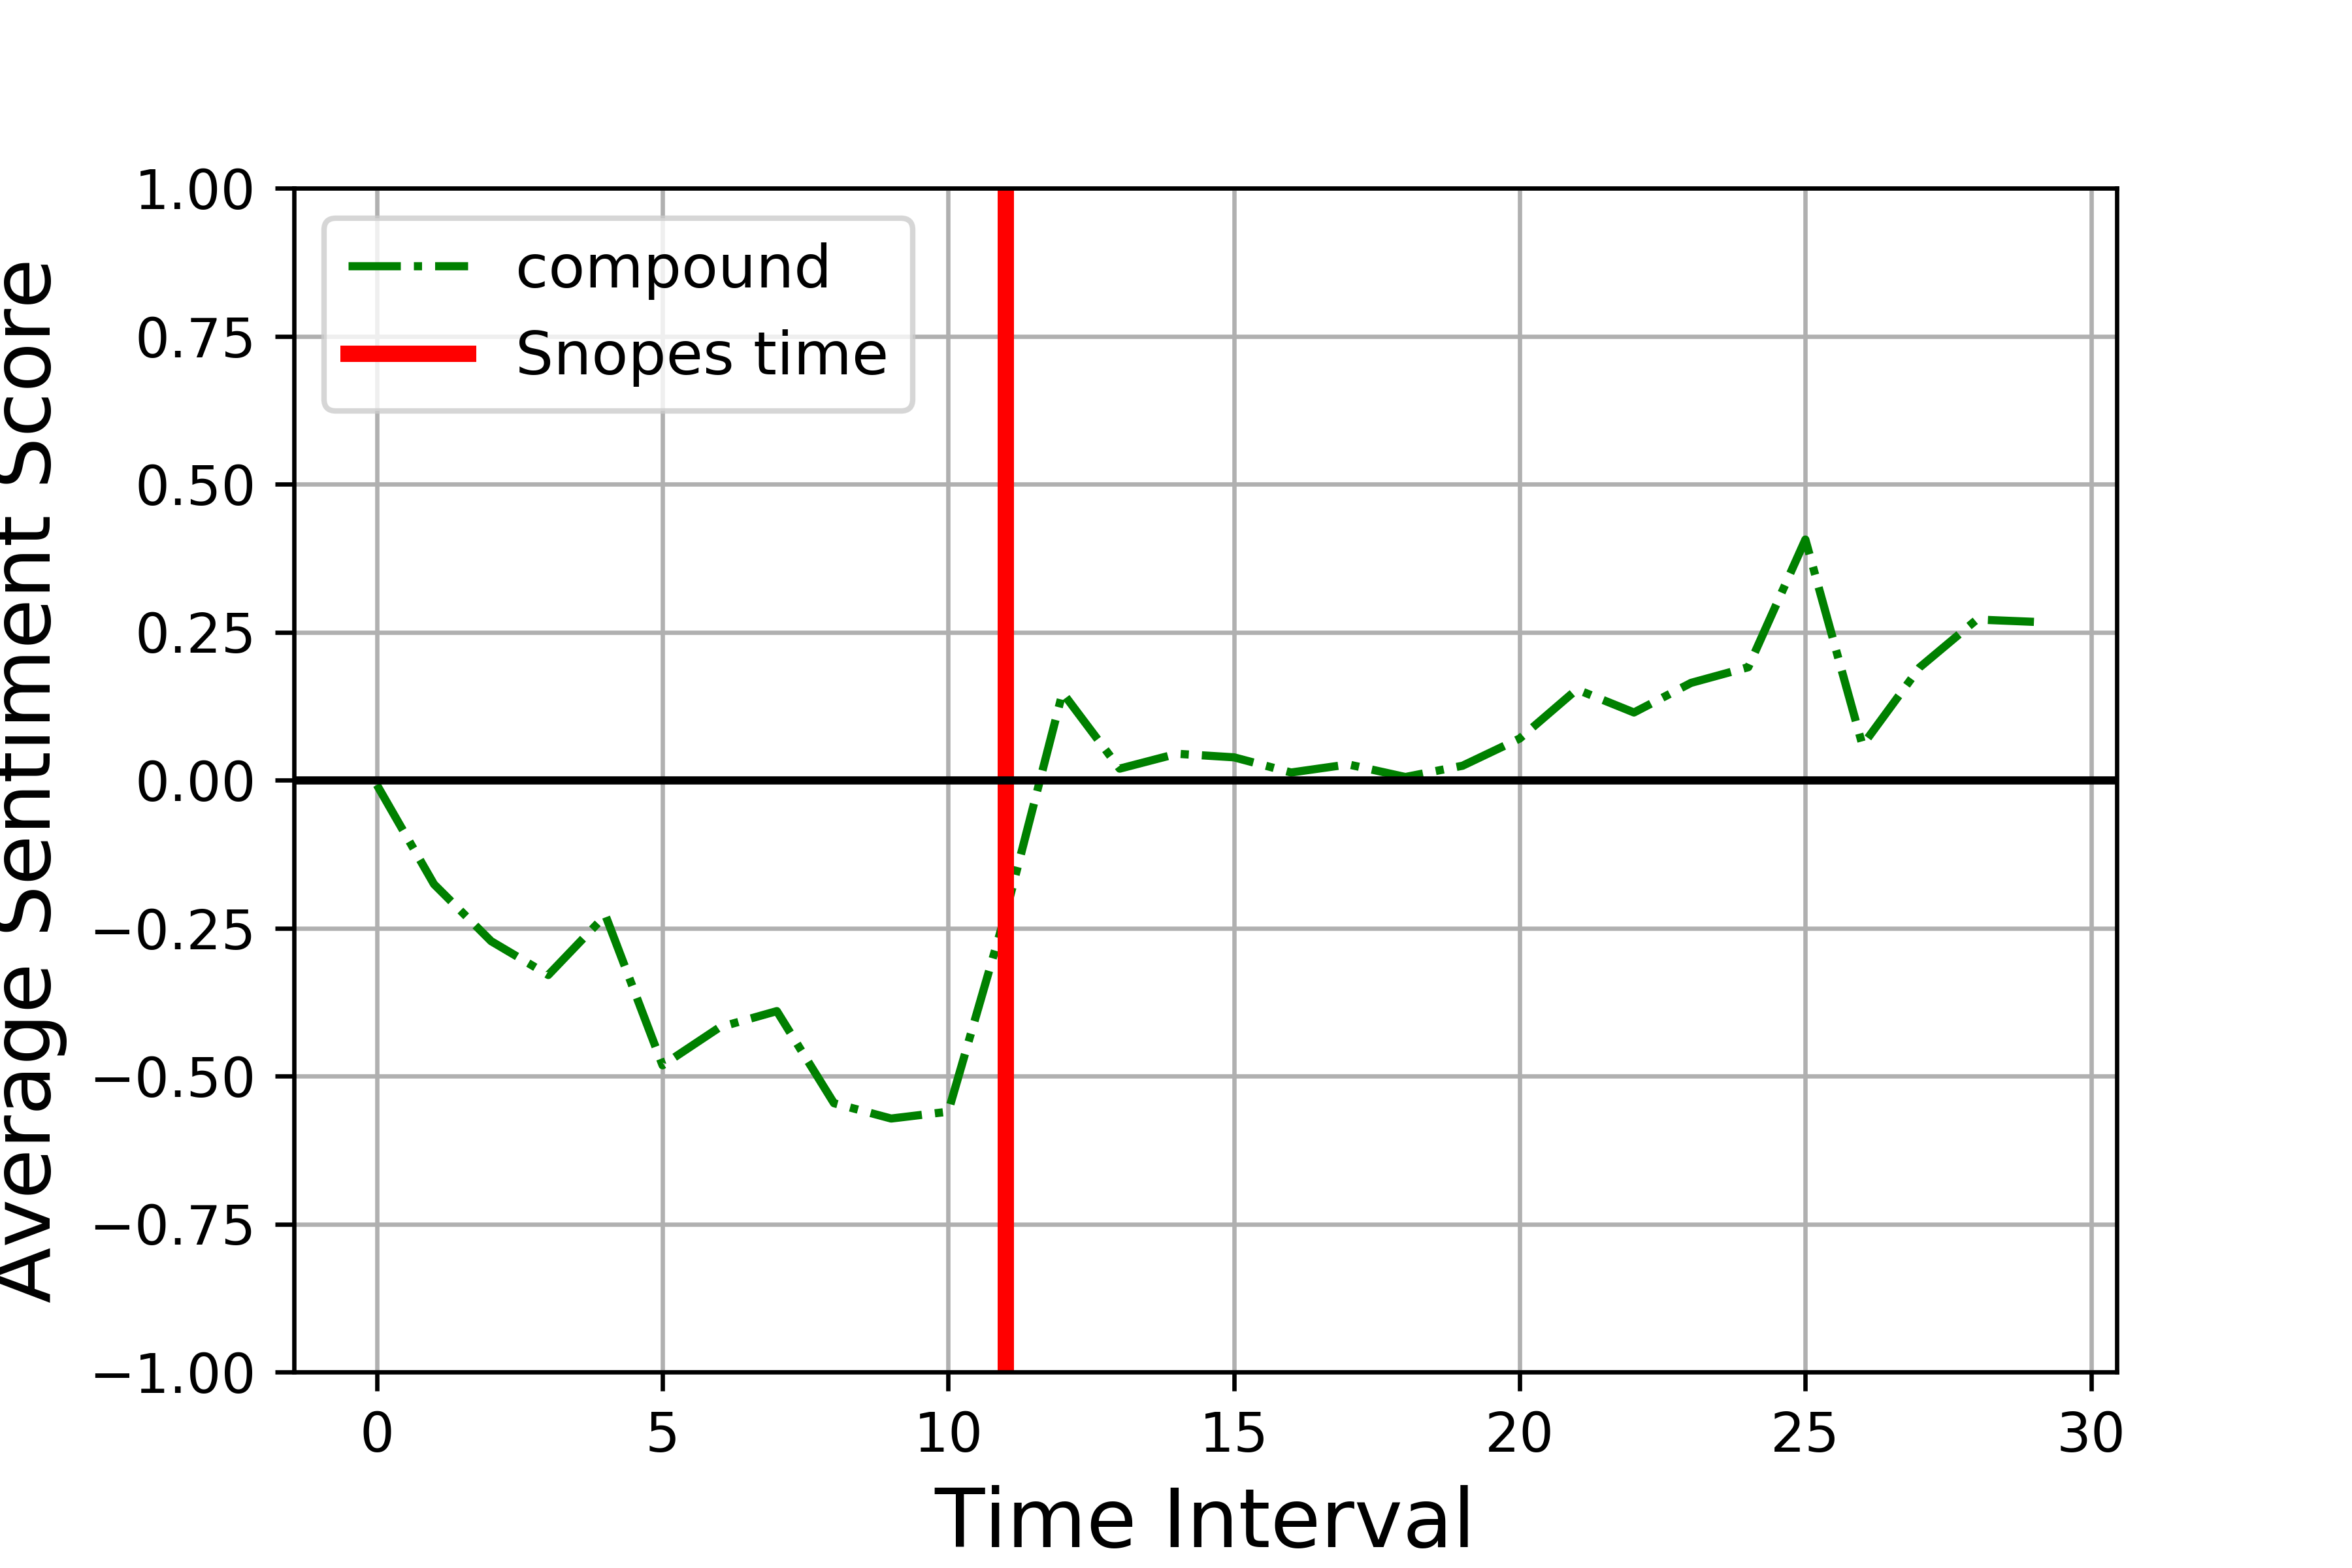
\includegraphics[width=3in]{figures/figure_6B.png}
			\label{fig:att_second_sub}
		}
		\caption{User's Belief Evolution of \textbf{True} Rumor Topic 'Trump Touches Glowing Orb in Saudi Arabia?'}
		\label{fig:attitude_A}
	\end{figure}
	
	\begin{figure}[htp]
		\centering
		\subfigure[User's Attitudes Evolution Over Time of Rumor topic]
		{
			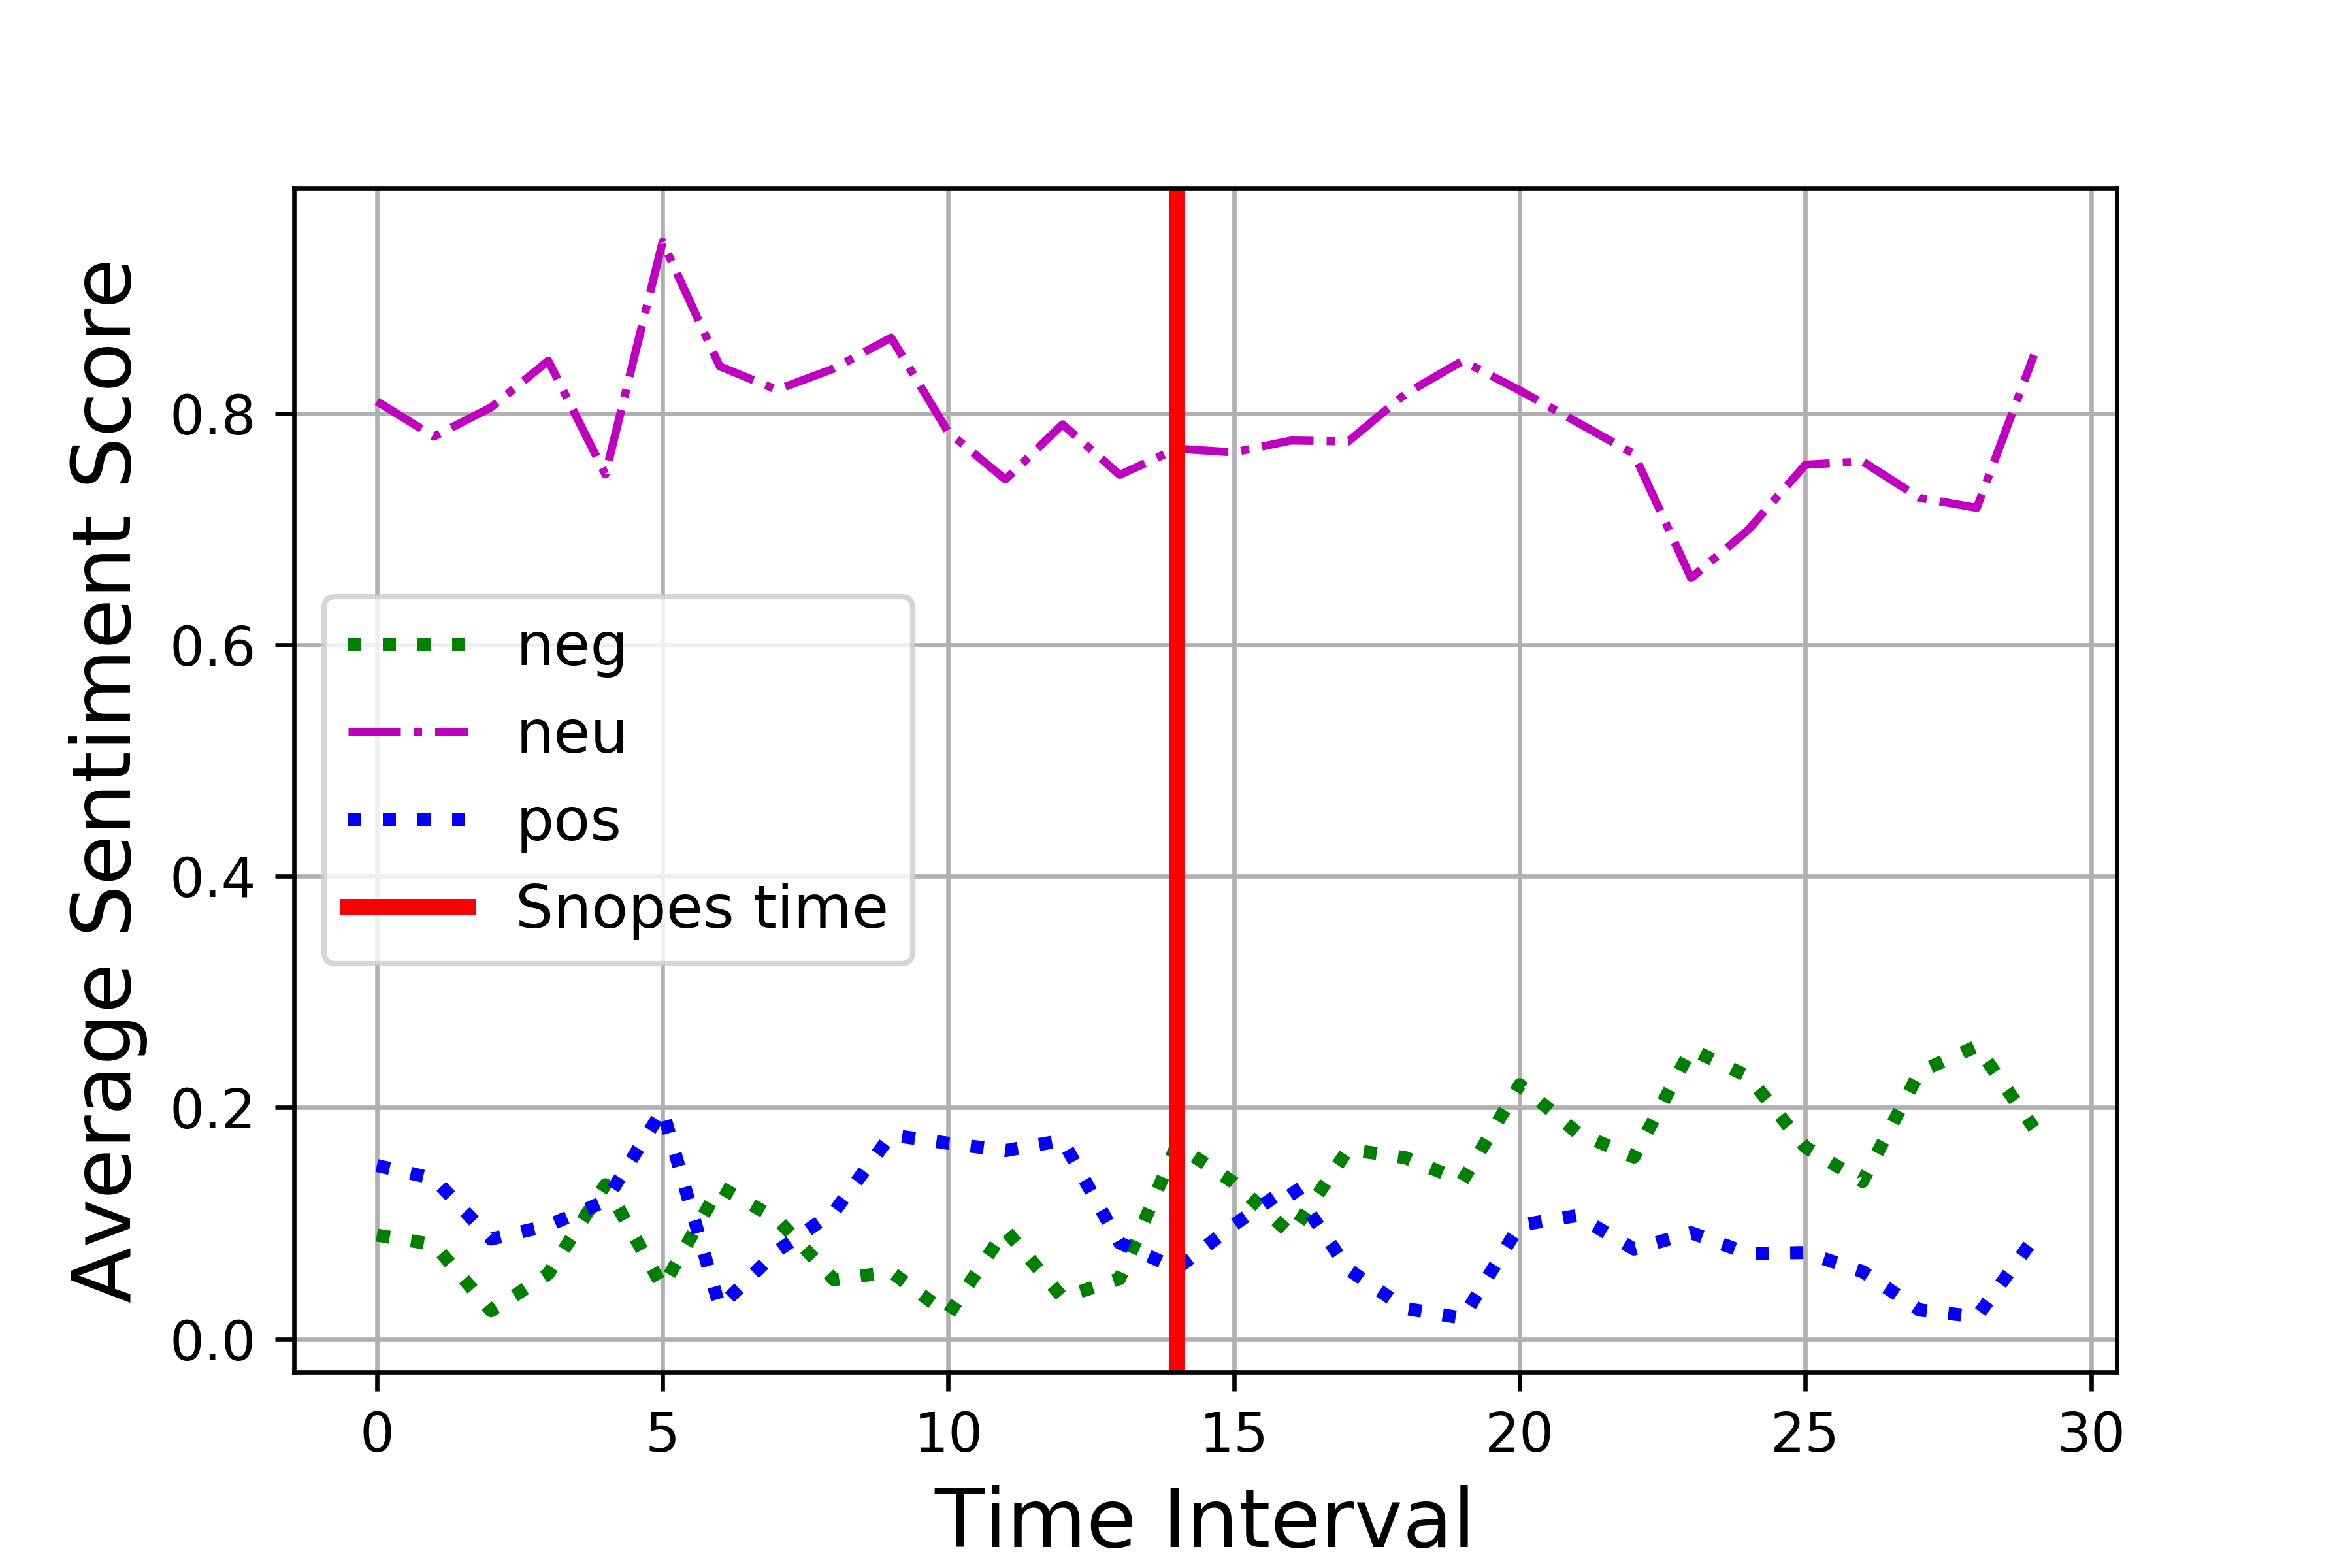
\includegraphics[width=3in]{figures/figure_7A.png}
			\label{fig:att_third_sub}
		}
		\subfigure[Overall Sentiment Score Change Over Time]
		{
			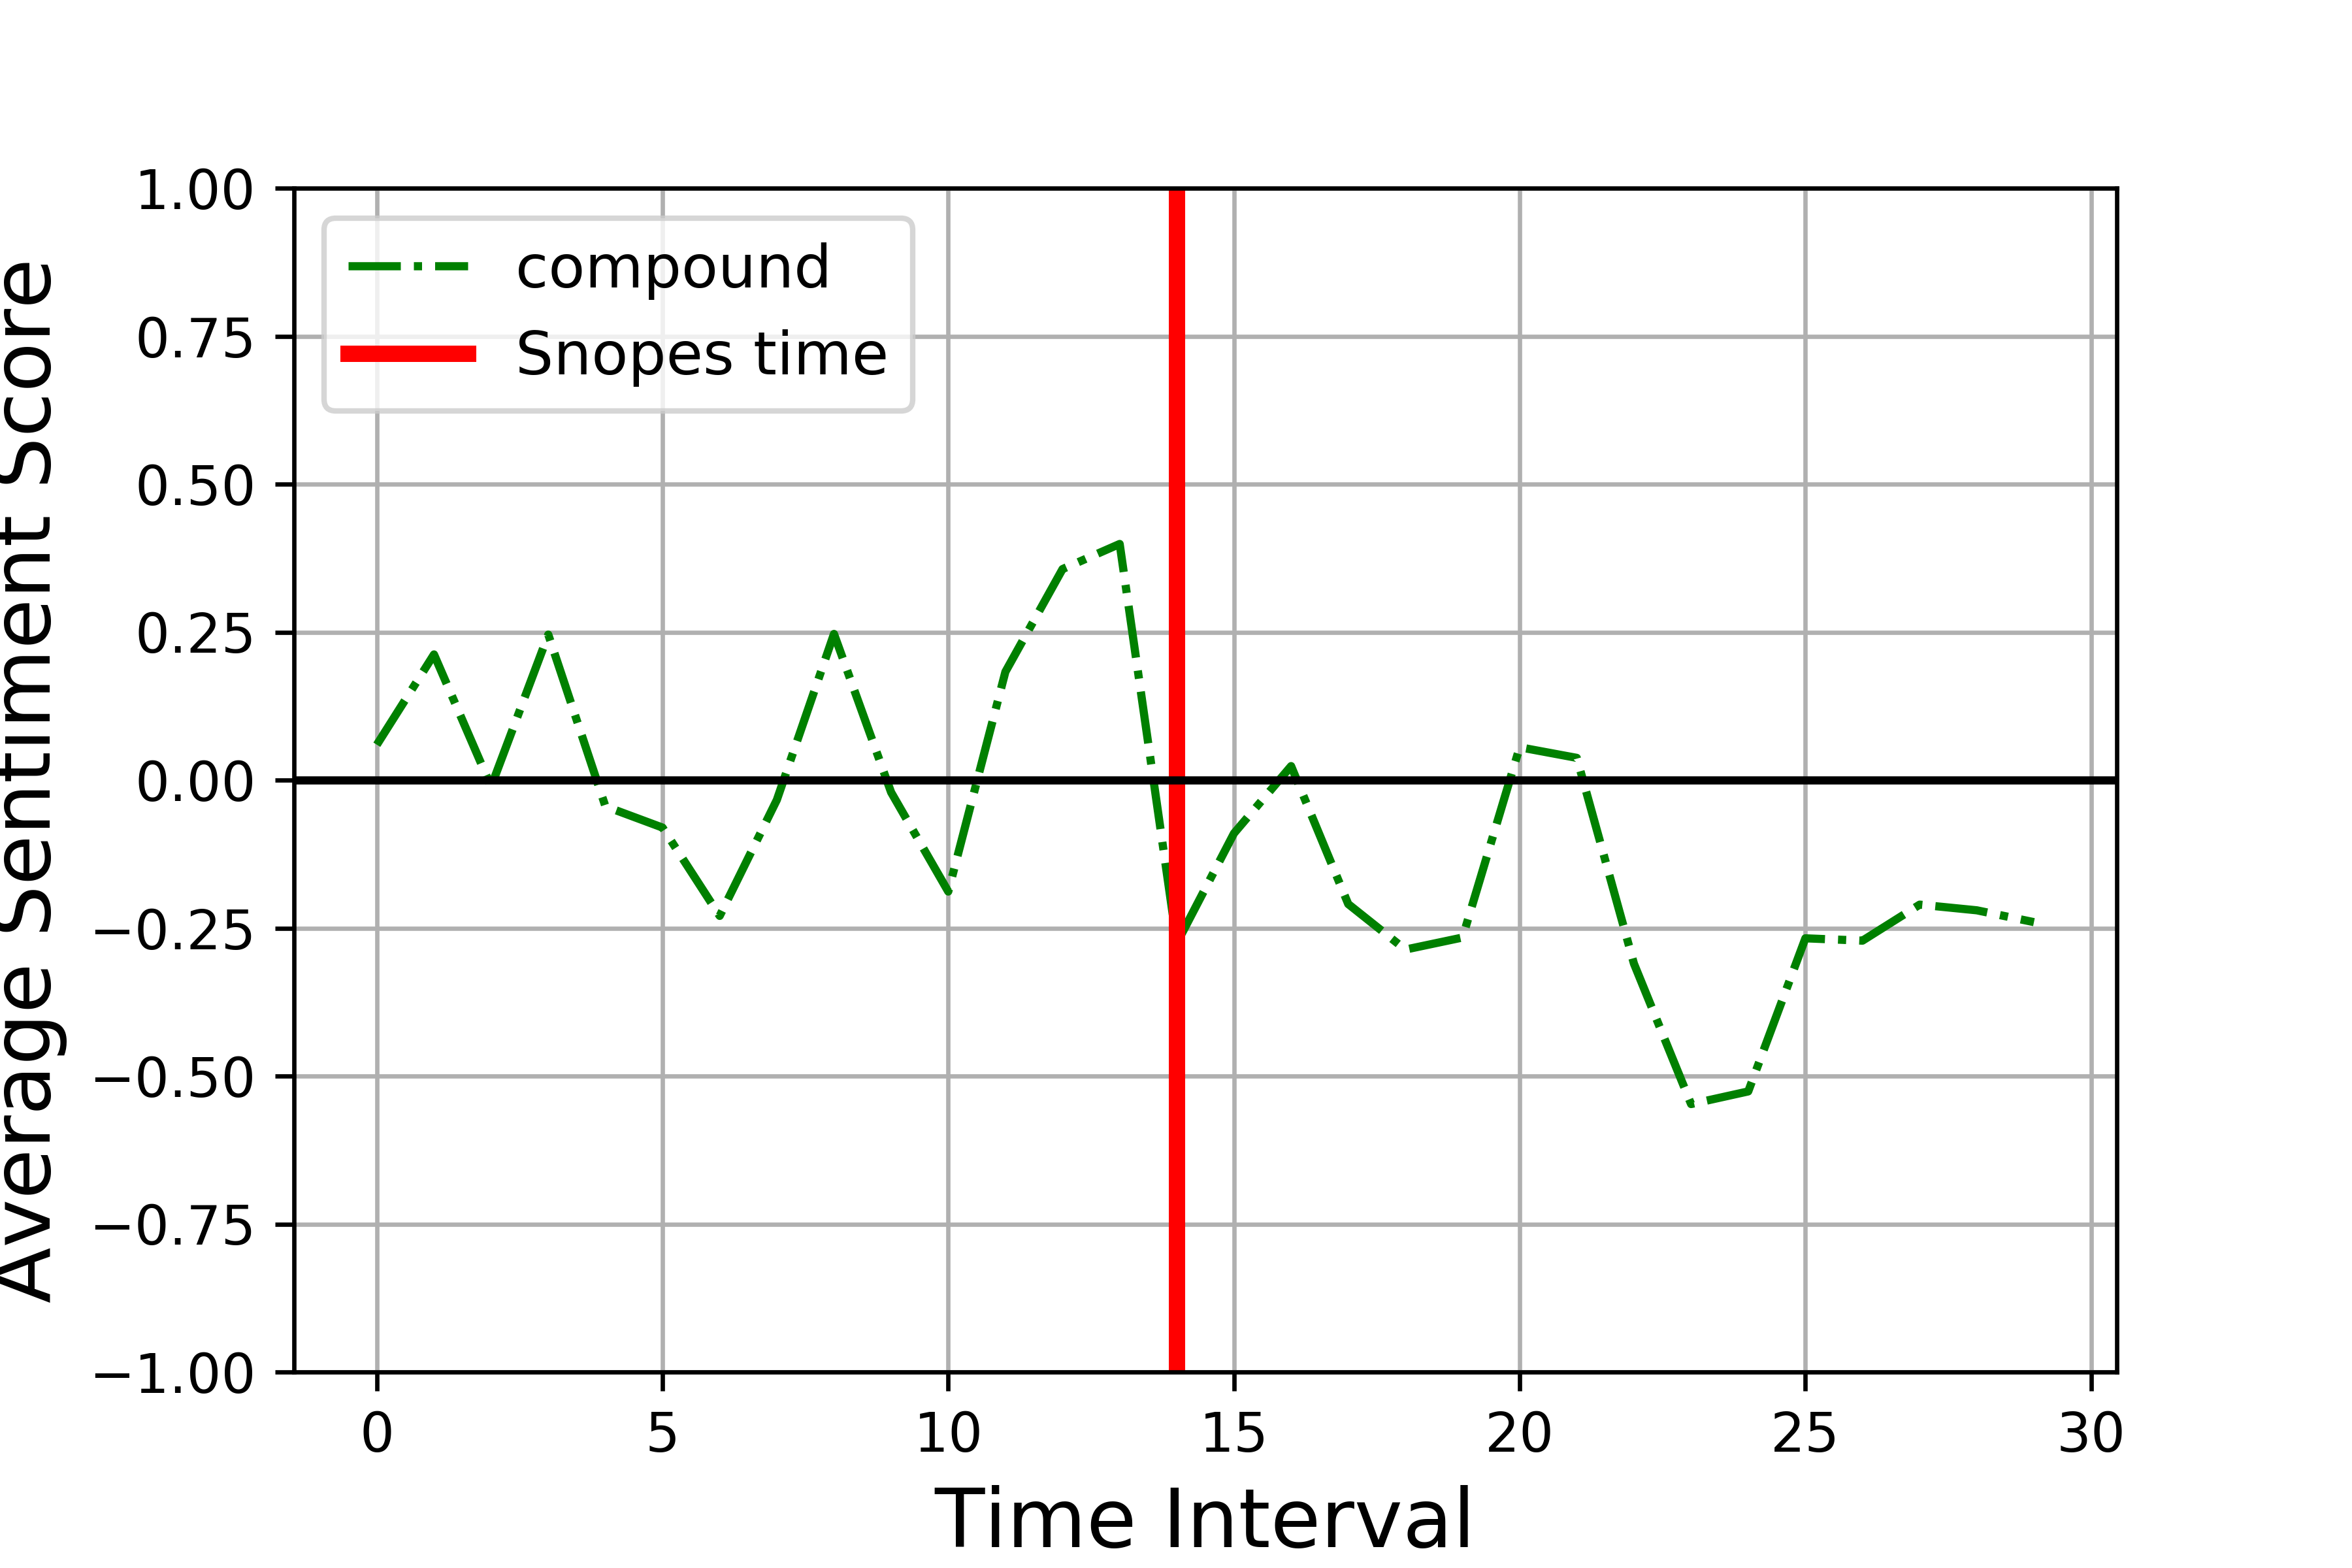
\includegraphics[width=3in]{figures/figure_7B.png}
			\label{fig:att_fourth_sub}
		}
		\caption{User's Belief Evolution of \textbf{False} Was the Passage of Obamacare Just as Secretive as GOP Efforts to Repeal It?'}
		\label{fig:attitude_B}
	\end{figure}
	
	Identifying belief in rumors can help reveal many semantic aspects of their origination and propagation \cite{zubiaga2016analysing}, and users' belief of a rumor may vary before and after the fact was checked. Moreover, users attitudes towards different veracity of rumors may also be different. 
	
	For the purpose of quantifying the user's belief towards a rumor topic, we categorize the user's belief into three different aspects: positive (supportive), negative (unsupportive), and neutral. The user's tweet which falls the 'neutral' category doesn’t express any specific statements or the user simply retweets a post of a rumor.
	
	We divided each tweet set based on its unique fact-checked time and extracted textual content from each tweet status. According to the NLTK's sentiment analysis package \cite{bird2009natural}, We calculated the sentiment score and an extra metric - compound value, which conveys the overall positive or negative user experience, of the tweet text for each belief category individually. We manifest the actual sentimental score for each category as well as the overall user's belief change over time. Besides, to study the user's belief evolution between the 'True' category and 'False' category, we compare user's belief change of two rumor topics that were verified as true and false, respectively (Fig. \ref{fig:attitude_A} and Fig. \ref{fig:attitude_B}). 
	
	As both figures show, the neutral sentiment value keeps on a high level around 0.8 steadily, which explains Twitter users hardly post polarized comments towards a rumor topic no matter what the veracity is, and most users disseminate information without revealing a particular belief about the topic. One feasible answer \cite{li2016user} is there is a character limit for each tweet which does not leave room for discussion or reflection on the rumor topic. 
	
	Fig. \ref{fig:att_first_sub} highlights the fact that the intervention of the Snopes message can effectively change the current belief trend. Before the fact-checking information, users generally expressed more negative reactions than positive reactions towards the true rumor that had not been verified yet. However, there has been a gradual rise of positive comments after the posting of debunking information, and the difference between the user's supportive and rejecting attitudes is significantly clear at the end of the propagation. At the propagation's final phase, the user's average positive feedback score rises up to 0.2 while negative feedback drops to 0.1. Fig. \ref{fig:att_second_sub} also demonstrates the overall change of user's belief of this 'true' rumor. The cumulative sentiment score keeps decreasing until the posting of the debunking article, and the final sentiment score ends at 0.25. 
	
	In contrast, Fig. \ref{fig:att_third_sub} shows the rumor topic, which has not been verified as false, draw more positive comments at its early stage of propagation. After the rumor was fact-checked and users realized the rumor is misinformation, the score of positive comments starts falling in each time interval. Meanwhile, there has been a gradual rise in negative comments. Regarding the overall compound score in Fig. \ref{fig:att_fourth_sub}, the unstable trend reveals the user's uncertainty of the rumor topic before the fact was checked. After the truth was revealed, the cumulative sentiment score fells to a lowest point of -0.5 and ends at -0.25 at the end of the diffusion. Besides, the generally downward trend in people's belief towards the misinformation after the fact was checked also reflects the effectiveness of the fact-checking website in mitigating online rumor's spread.
	
	\section{The Impact of Debunking Information}
	In order to further verify if fact-checking websites have the ability to mitigate the spread of rumor on social media, we design a learning task attempting to separate groups of tweets before and after presenting its debunking information. High accuracy of machine learning models' result indicates there is a distinction between a rumor's different propagation phases.
	
	\subsection{Experiment Setup}
	We further conduct analysis on the 74 rumor topics appearing from April to September in 2017 with the machine learning approach. Since diffusion of an online rumor has its continuous and increasing characteristics, and the overall evolution of an online rumor may take up to several years or only a few days. Therefore, in order to find variations in rumor propagation's different phases, we evenly divide each topic into five intervals based on the earliest and the latest posted tweet time, and all tweets of a topic, as well as the fact-checking information, fall into split time intervals. Each time interval of a rumor topic is labeled based on whether the create-time of debunking message is in the time interval. Then, for quantifying each time interval and utilizing features from each time interval, we vectorize each time interval. Details of features will be listed in the next section.
	
	Our object in this paper is to study the existence of impact by fact-checking information and the potential effects brought by debunking information in the spread of online rumors. To address this problem by machine learning approach, we transform this problem as a classification and clustering problem with the supervised and unsupervised methods, respectively. 
	
	For unsupervised learning methods, if clustering models can accurately cluster non-Snopes intervention intervals and Snopes intervention intervals, the impact of the fact-checking message in the dissemination can be established. On the other hand, since each interval vector has its label of whether it's intervened by the fact-checking message, we use linear classifiers, including Support Vector Machine (SVM), logistic regression, and k-nearest neighbors, to separate each time intervals. If linear classification models can achieve remarkable results, we can prove the fact-checking message can effectively impact the rumor propagation process since different time intervals are linearly separable.
	
	\subsection{Experiment Methods and Results}
	We proceed by describing factors that reflects the spread of a rumor with the time change. For each divided time interval, we split it into ten smaller intervals based on the earliest and latest tweets create time in order to represent the spread pattern in unit time. According to Cheng \textit{et al.}'s summary of factors driving cascade growth \cite{cheng2014can}, we conclude two major features: \textbf{Content Features} and \textbf{Temporal Features}.
	
	\begin{itemize}
		\item \textbf{Content Features}\\
		The first natural factor contributing to the spread of online rumor is its own content; in other words, the user would share or comment a tweet because there is an attraction point on those inflammatory tweet's contents \cite{cheng2014can, kumar2018false}. Typically, a tweet is composed of the main texts and self-generated labels, namely hashtags. The linguistic features extracted from text can reflect a user's emotion change towards a rumor. Kwon suggests a list of user's emotional change in the process of rumor difussion \cite{kwon2013prominent}: rumors were significantly less like to contain emotional comments at its early phase because of user's uncertainty regarding an online rumor. Once it has been linked with a verifying article, people start to take a cognitive action to the rumor related content. 
		
		We consider all of the text and hashtag information in a given time interval, and we vectorize the textual information with TF-IDF techniques after removing stop words and uncommon characters. In addition, as described in last section, we take into account tweet's sentimental score as a joint feature. \\
		
		\item \textbf{Temporal Features}\\
		Properties related to the evolution of rumor cascades were shown to be the most important features in predicting online content popularity \cite{ma2013predicting}, and our statistics in the previous section also shows that the posting of debunking information can disturb the growth trend of rumor cascade's number and average size. According to \cite{vosoughi2018spread, kumar2018false, shao2016hoaxy}, online rumors generally spread rapidly and widely at its early propagation phase. And the expansion of online rumor would get controlled within 10 to 20 hours after fact-checking media post the debunking information. Therefore, the change in the number of tweets and users may reflect whether this interval is influenced by the fact-checking message.
		
		We thus characterize a number of temporal properties of cascade diffusion over time. In particular, we consider the change in the total number of tweets and users per time unit, we also calculate the number of newly emerged tweets between each time unit. 
		\\
		
	\end{itemize}
	
	We choose three representative linear classification model: Support Vector Machine (SVM), Logistic Regression (LR), and k Nearest Neighbors (kNN). We wish linear classifiers can learn different propagation patterns from our sample data with acceptable accuracy. Correspondingly, we select three clustering models: K-Means, Spectral Clustering, and Agglomerative Clustering. The reason for choosing the above models is we can regulate there are only two clusters among all intervals. If clustering models can successfully separate whether the fact-checking information is posted in the interval, the effectiveness of fact-checking information can also be proved. 
	
	Table \ref{tab1e:machinelearning} shows the selected supervised and unsupervised learning model's performance by using two feature. Generally, temporal feature performed better. 
	
	\begin{table}[htbp]
		\begin{center}
			\caption{Performance of Each Models}
			\begin{tabular}{|c|c|c|}
				\hline \\[-1em]
				\multirow{2}{*}{Name}    & \multicolumn{2}{|c|}{Performance} \\ \cline{2-3} \\[-1em]
				& Textual        & Temporal        \\ \hline \\[-1em]
				\multicolumn{3}{|c|}{Supervised Learning Approach}          \\ \hline \\[-1em]
				SVM                      & 0.81439        & 0.83432         \\ \hline \\[-1em]
				Logistic Regression      & 0.80241        & 0.84784         \\ \hline \\[-1em]
				k Nearest Neighbors      & 0.81722        & 0.78378         \\ \hhline{|=|=|=|} \\[-1em]
				\multicolumn{3}{|c|}{Unsupervised Learning Approach}        \\ \hline \\[-1em]
				K-Means                  & 0.59868        & 0.68919         \\ \hline \\[-1em]
				Spectral Clustering      & 0.67512        & 0.64162         \\ \hline \\[-1em]
				Agglomerative Clustering & 0.65123        & 0.64595         \\ \hline
			\end{tabular}
			\label{tab1e:machinelearning}
		\end{center}
	\end{table}
	
	
	\section{Conclusion}
	This study set out to examine the function of fact-checking information in mitigating online rumors. We traced top 216 rumor topics affiliated with over four hundred thousand tweets on Twitter and monitored their propagation pattern with the intervention of fact-checking information. Characteristics' change of rumor cascades, as well as the user's sentiment change towards the introduction of fact-checking information, were analyzed. The results of this study indicate that debunking message can not only mitigate the spread of rumor on the social network, user's attitude would also switch oppositely with the posting of debunking message. 
	
	
	
	
	\bibliographystyle{IEEEtran}
	\bibliography{clingbib}
	
\end{document}
